\documentclass[CJK,aspectratio=169]{beamer}  %aspectratio控制页面的宽高比,16:9充满屏幕
\usepackage{beamerthemesplit}
\usetheme{Warsaw}
\usepackage{ctex} %中文字体设置
\usepackage{subfig}
\usepackage{amssymb,amsmath,mathtools}
\usepackage{amsfonts,booktabs}
\usepackage{lmodern,textcomp}
\usepackage{color}
\usepackage{tikz}
%\usepackage[latin1]{inputenc}
\usepackage{natbib}
\usepackage{multicol}
\usepackage{caption} 
\usepackage{graphicx}
\usepackage{makecell}                 % 三线表-竖线
\usepackage{booktabs}                 % 三线表-短细横线

\logo{
\includegraphics[height=0.5cm]{picture/badge-white_160x160.png}} % 将 logo 放置在左上角,调整高度为 1cm

\begin{document}
	
	\title{工作汇报}
	\author[Gu Rui (LZU)]{Gu Rui \inst{1}}
	\institute[*]{\inst{1} School of Information Science and Engineering,\\
		Lanzhou University\\
		npukujui11@gmail.com}
	
	\newcommand{\monthname}[1][\the\month]{%
		\ifcase#1\or
		January\or February\or March\or April\or May\or June\or
		July\or August\or September\or October\or November\or December\fi}
		
	\renewcommand{\today}{\monthname[\the\month] \the\day, \the\year}
	\renewcommand{\figurename}{Figure}
	\renewcommand{\tablename}{Table}
	\renewcommand{\refname}{References}
	\date{\today}
	
	\begin{frame}
		\titlepage
	\end{frame}
	
	\begin{frame}
		\begin{multicols}{2}
			\small \tableofcontents
		\end{multicols}
	\end{frame}
	
%	\begin{frame} \transblindshorizontal<1>  %百叶窗效果
%		
%		\begin{itemize}
%			\item <1> {\bf 章节4}
%			\begin{itemize}
%				\item {章节4.1}
%				\begin{itemize}
%					\item {4.1.2}
%				\end{itemize}
%			\end{itemize}
%			
%		\end{itemize}		
%	\end{frame}
	
	\section{模型结构}
	
	\subsection{Architecture}
	
	\begin{frame}
		\begin{figure}[htbp]
			\begin{center}
				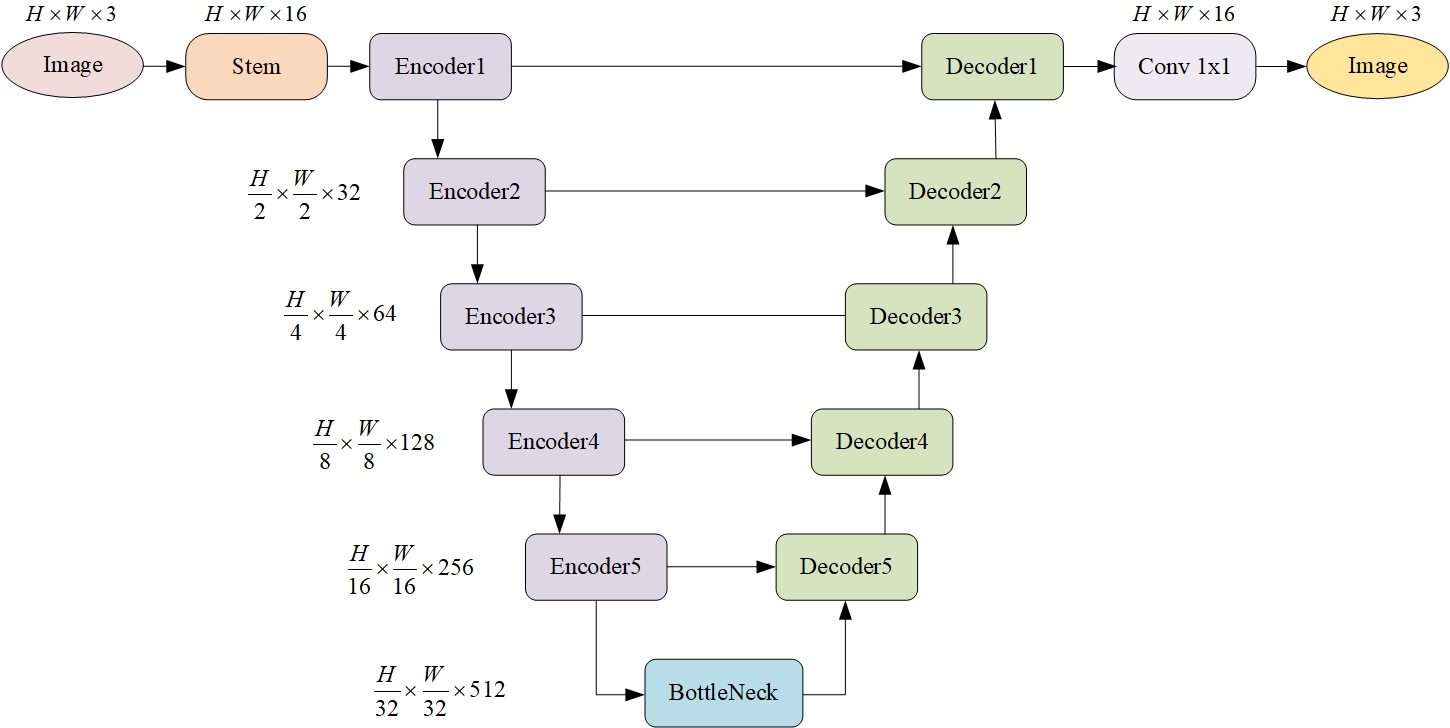
\includegraphics[width=0.8\textwidth]{picture/LLIE/My Architecture/ULite_Enhance}
			\end{center}
		\end{figure}
		
		\begin{minipage}{.45\textwidth}
			\textbf{\tiny Architecture}
			\begin{itemize}\tiny
				\item [-] U-Net
				% 通过一个简单的 U-Net 去对外观建模,可以理解成先简单地学习到一个正常光照的 coarse version。其中,损失函数为一个重建损失加感知损失。
				
				\item [-] Structure-Aware Feature Extractor
				% 对于结构信息建模部分,借鉴了 GAN prior 的思路,但是不用预训练的GAN 模型。这里设计到一个结构特征的提取Structure-Aware Feature Extractor (SAFE)
				
				\item [-] Structure-Guided Enhancement Module
				% 为了利用得到的结构图来提高外观,作者设计了一个结构导向增强模块 Structure-Guided Enhancement Module(SGEM模块)初始外观建模结果。在 SGEM 中,根据结构映射生成空间自适应核和归一化参数。然后,对SGEM 解码器的每一层的特征进行空间全处理y−自适应卷积和归一化。虽然 SGEM 的整体架构采用了一个简单的U-Net 的形式,但它可以有效地增强原始的外观。
			\end{itemize}
		\end{minipage}
		\begin{minipage}{.45\textwidth}
			\textbf{\tiny Edge Detection}
			\begin{itemize}\tiny
				\item [-] Too few datasets for extracting edge information
				% 论文指出低光数据集图片较少,所以结构信息提取模块的训练会受限,因此作者引入其他结构信息提取的数据集做额外训练可以进一步提升performance
				
				\item [-] Semantic maps and depth maps
				% 作者提出除了边缘结构图作为引导信息,也可以使用其他特征,比如语义图( Ours with SEG.)和深度图( Ours with Dep.),总体表现没有边缘图好,但是也比一些现有的增强方法好。
				
				\item [-] Input image or initial enhanced image
				% 作者没有说 Appearance Modeling 的结果去提取边缘会达到什么效果?
				
				% 此外作者做消融实验的过程中,使用一个 SOTA 边缘提取网络代替论文中的structural modeling 模块(但是感觉在低光照下很难提取到有效的边缘,合理点的话需要先对输入亮度增强一下)
			\end{itemize}
		\end{minipage}
	\end{frame}
	
	\subsection{Sub-Model}
	
	\begin{frame}
		
		\begin{figure}[htbp]
			\begin{center}
				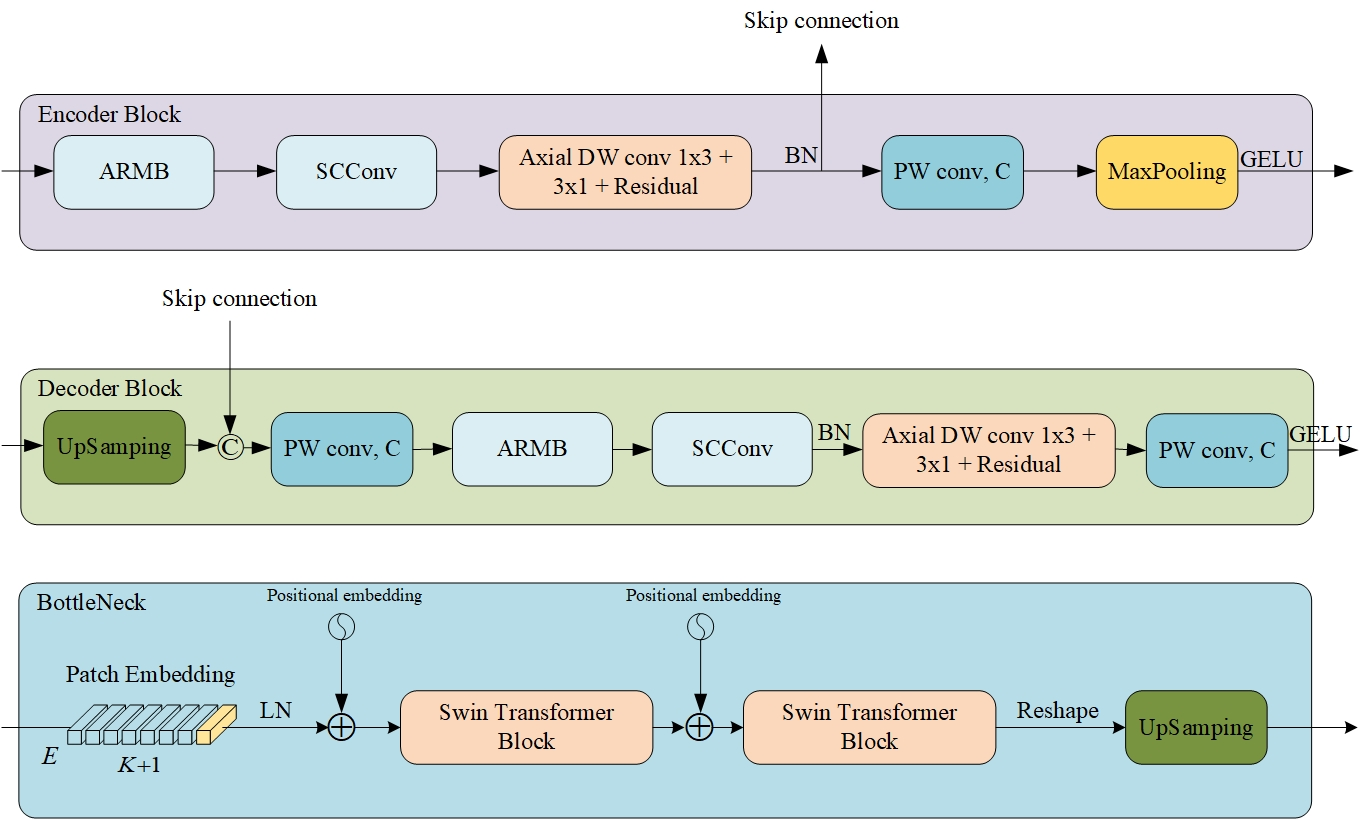
\includegraphics[width=0.8\textwidth]{picture/LLIE/My Architecture/Encoder_Decoder}
			\end{center}
		\end{figure}

	\end{frame}
	
%	\begin{frame}
%		\section{Literature Review}
%		Study hard and make progress every day. % 第一等级
%		\begin{itemize} 
%			\item Study hard and make progress every day. % 第二等级
%			\begin{itemize}
%				\item Study hard and make progress every day. % 第三等级
%				\begin{itemize}
%					\item Study hard and make progress every day. % 第四等级
%				\end{itemize}
%			\end{itemize}
%		\end{itemize}
%	\end{frame}
	
	\subsection{Swin Transformer Block}
	
	\begin{frame}
		
		\begin{figure}[htbp]
			\begin{center}
				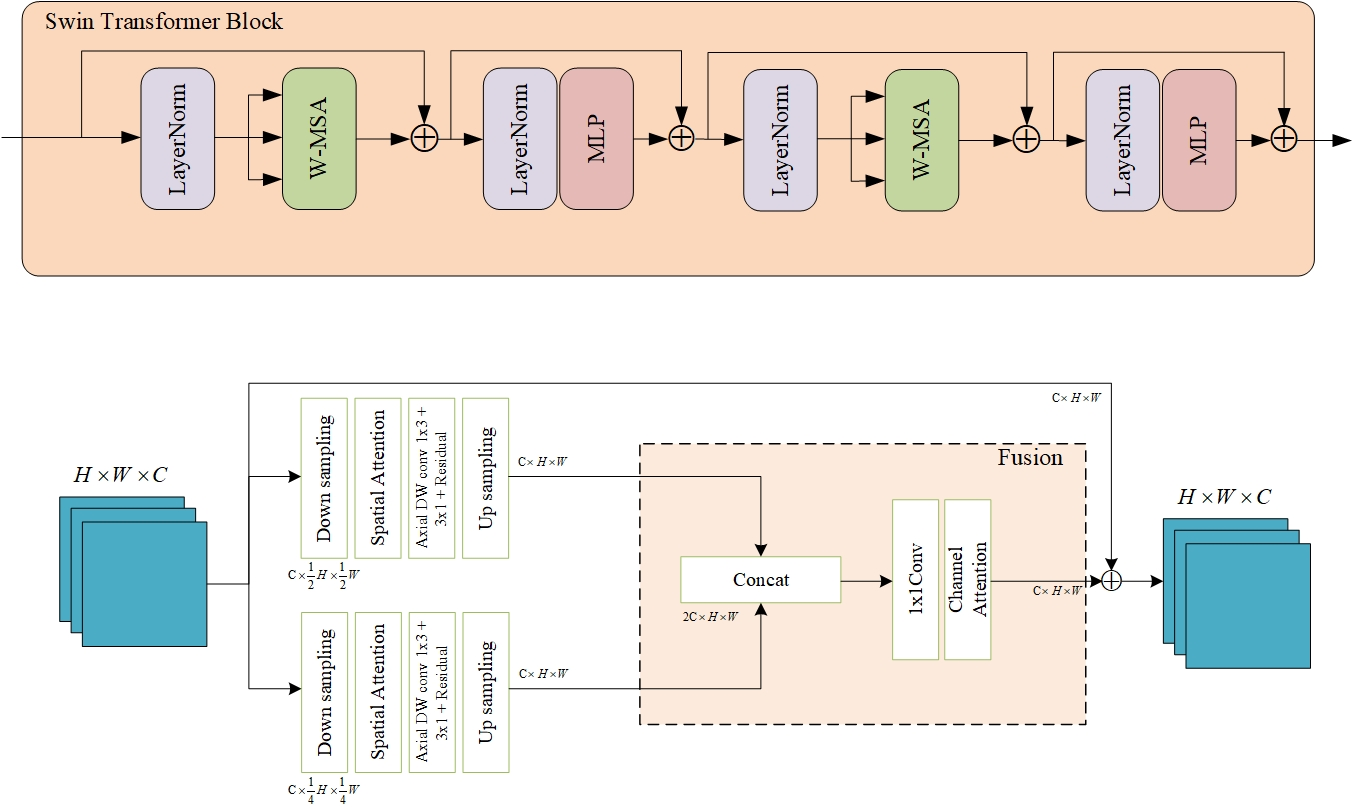
\includegraphics[width=0.8\textwidth]{picture/LLIE/My Architecture/Swin Transformer}
			\end{center}
		\end{figure}
			
	\end{frame}
	
	\subsection{Structure Modeling and Guidance}
	
	\begin{frame}
		
		Low-Light Image Enhancement via Structure Modeling and Guidance\textcolor{blue}{\citep{xu2023low}}
		
		\begin{itemize} 
			\item \textbf{Background}
			
			\item[\checkmark] Appearance and structural information defects of the image.
				
			% 由于低光照条件下的图像容易受到噪声的影响,现有的低光图像增强方法往往无法同时处理图像的外观和结构信息,导致结果过度增强或者不真实。
			\vspace{.3cm}
			\item[\checkmark] Current methods (based encoder and decoder network) \textcolor{blue}{\citep{rana2021edge}}\textcolor{blue}{\citep{zhu2020eemefn}} that use structural information to boost enhancement do not work well 
			
			% 在暗区域中加入敏感边缘先验可以降低优化外观重构时的不适定程度。这些框架使用基于编码器-解码器的网络和回归损失执行结构建模。然而,由于能见度和噪声严重不足导致的暗区不确定性,相应的结构建模结果并不令人满意。
			
		\end{itemize}
		
		\begin{itemize}
			\item \textbf{Contribution}
			
			\item[\checkmark] A Gan Loss-based model goes out to model the structural information.
			
			% 论文提出了一种基于 GAN Loss 的模型去对结构信息建模,通过获得的结构信息指导增强。
			\vspace{.3cm}
			\item[\checkmark] It is difficult to extract good structural information from the low-illumination images.
			
			% 从低光图像中很难提取到好的结构信息,但是论文中提出的方法提取到的结构信息会好很多,并且用于指导图像增强信息。
		\end{itemize}	
		
	\end{frame}
	
	\begin{frame}
		
		\begin{figure}
			\centering
			\begin{minipage}{.25\textwidth}
				\centering
				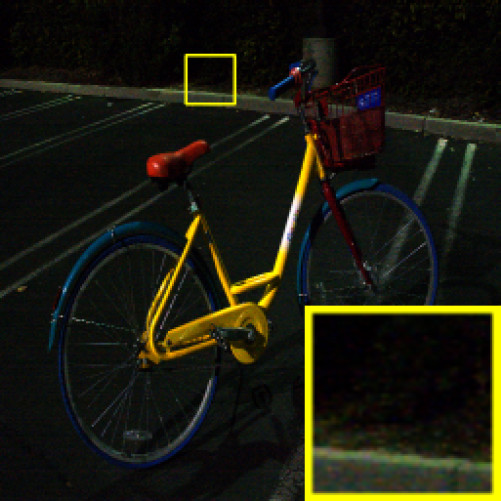
\includegraphics[width=.8\linewidth]{picture/LLIE/Structure Modeling and Guidance/Input}
				\captionsetup{font=scriptsize}
				\label{fig: SMG_Input}
				\caption*{Input}
			\end{minipage}
			\begin{minipage}{.25\textwidth}
				\centering
				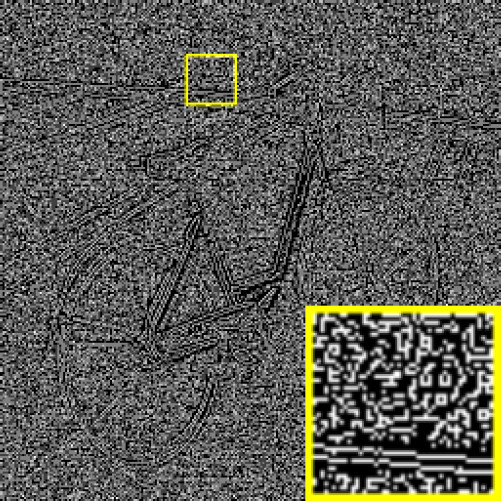
\includegraphics[width=.8\linewidth]{picture/LLIE/Structure Modeling and Guidance/Structure of (a)}
				\captionsetup{font=scriptsize}
				\label{fig: Structure of (a)}	
				\caption*{Structure of (a)}
			\end{minipage}
			\begin{minipage}{.25\textwidth}
				\centering
				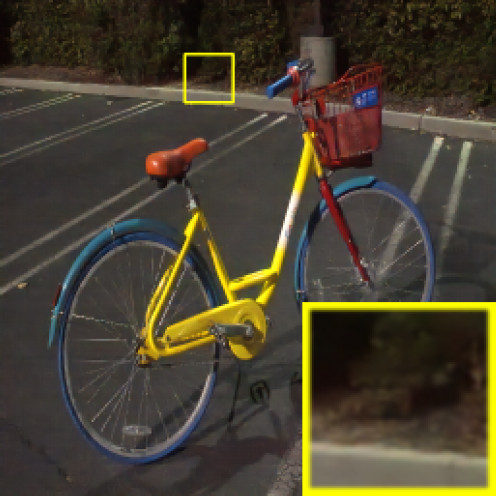
\includegraphics[width=.8\linewidth]{picture/LLIE/Structure Modeling and Guidance/SNR (CVPR 2022)}
				\captionsetup{font=scriptsize}
				\label{fig: SNR (CVPR 2022)}	
				\caption*{SNR (CVPR 2022)}
			\end{minipage}
			\begin{minipage}{.25\textwidth}
				\centering
				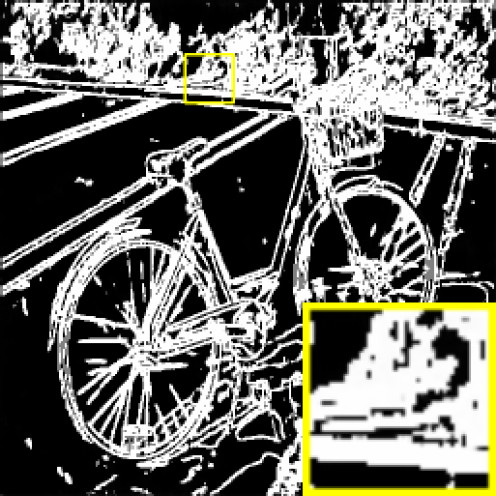
\includegraphics[width=.8\linewidth]{picture/LLIE/Structure Modeling and Guidance/Structure Modeling}
				\captionsetup{font=scriptsize}
				\label{fig: Structure Modeling}	
				\caption*{Structure Modeling}
			\end{minipage}
			\begin{minipage}{.25\textwidth}
				\centering
				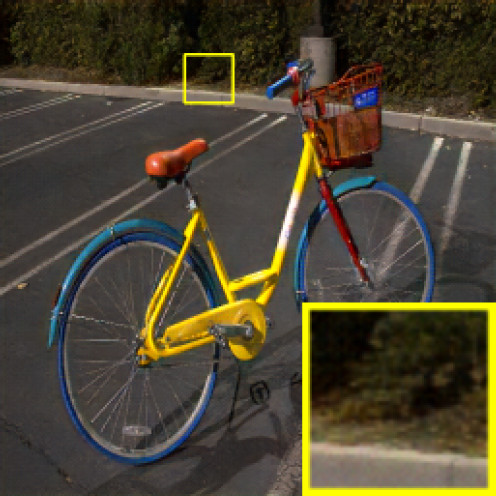
\includegraphics[width=.8\linewidth]{picture/LLIE/Structure Modeling and Guidance/Ours}
				\captionsetup{font=scriptsize}
				\label{fig: SMG_Ours}	
				\caption*{Ours}
			\end{minipage}
			\begin{minipage}{.25\textwidth}
				\centering
				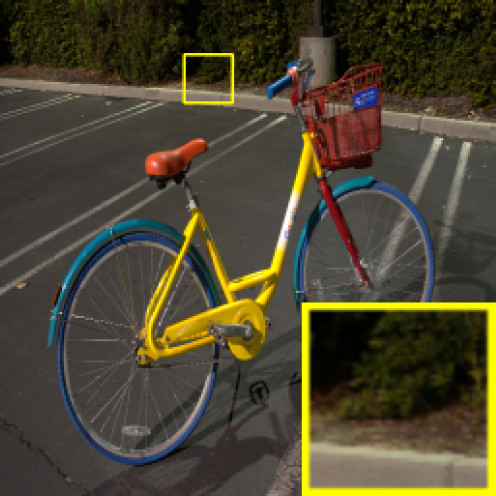
\includegraphics[width=.8\linewidth]{picture/LLIE/Structure Modeling and Guidance/Ground Truth}
				\captionsetup{font=scriptsize}
				\label{fig: Ground Truth}	
				\caption*{Ground Truth}
			\end{minipage}
			\captionsetup{font=scriptsize}
			\caption{
				\label{fig: Structure Information}
				A challenging low-light frame (a), from SID-sRGB\cite{chen2018learning},
				enhanced by a SOTA method (c) and our method (e). Our method
				can synthesize the structure map (d) from the input image, leading
				to clearer details, more distinct contrast, and more vivid color. Although
				(c) has high PSNR as 28.17, its SSIM is low as 0.75. Ours
				achieves high scores for both dB and SSIM, as 28.60dB and 0.80.
			}
		\end{figure}
		% 作者的模型 PSNR 和 SSIM 得分在 LOL-v2 数据集中很高。
		% 作者的方法可以从输入图像中合成结构图 Structure Modeling
	\end{frame}
	
	\begin{frame}
		\begin{figure}[htbp]
			\begin{center}
				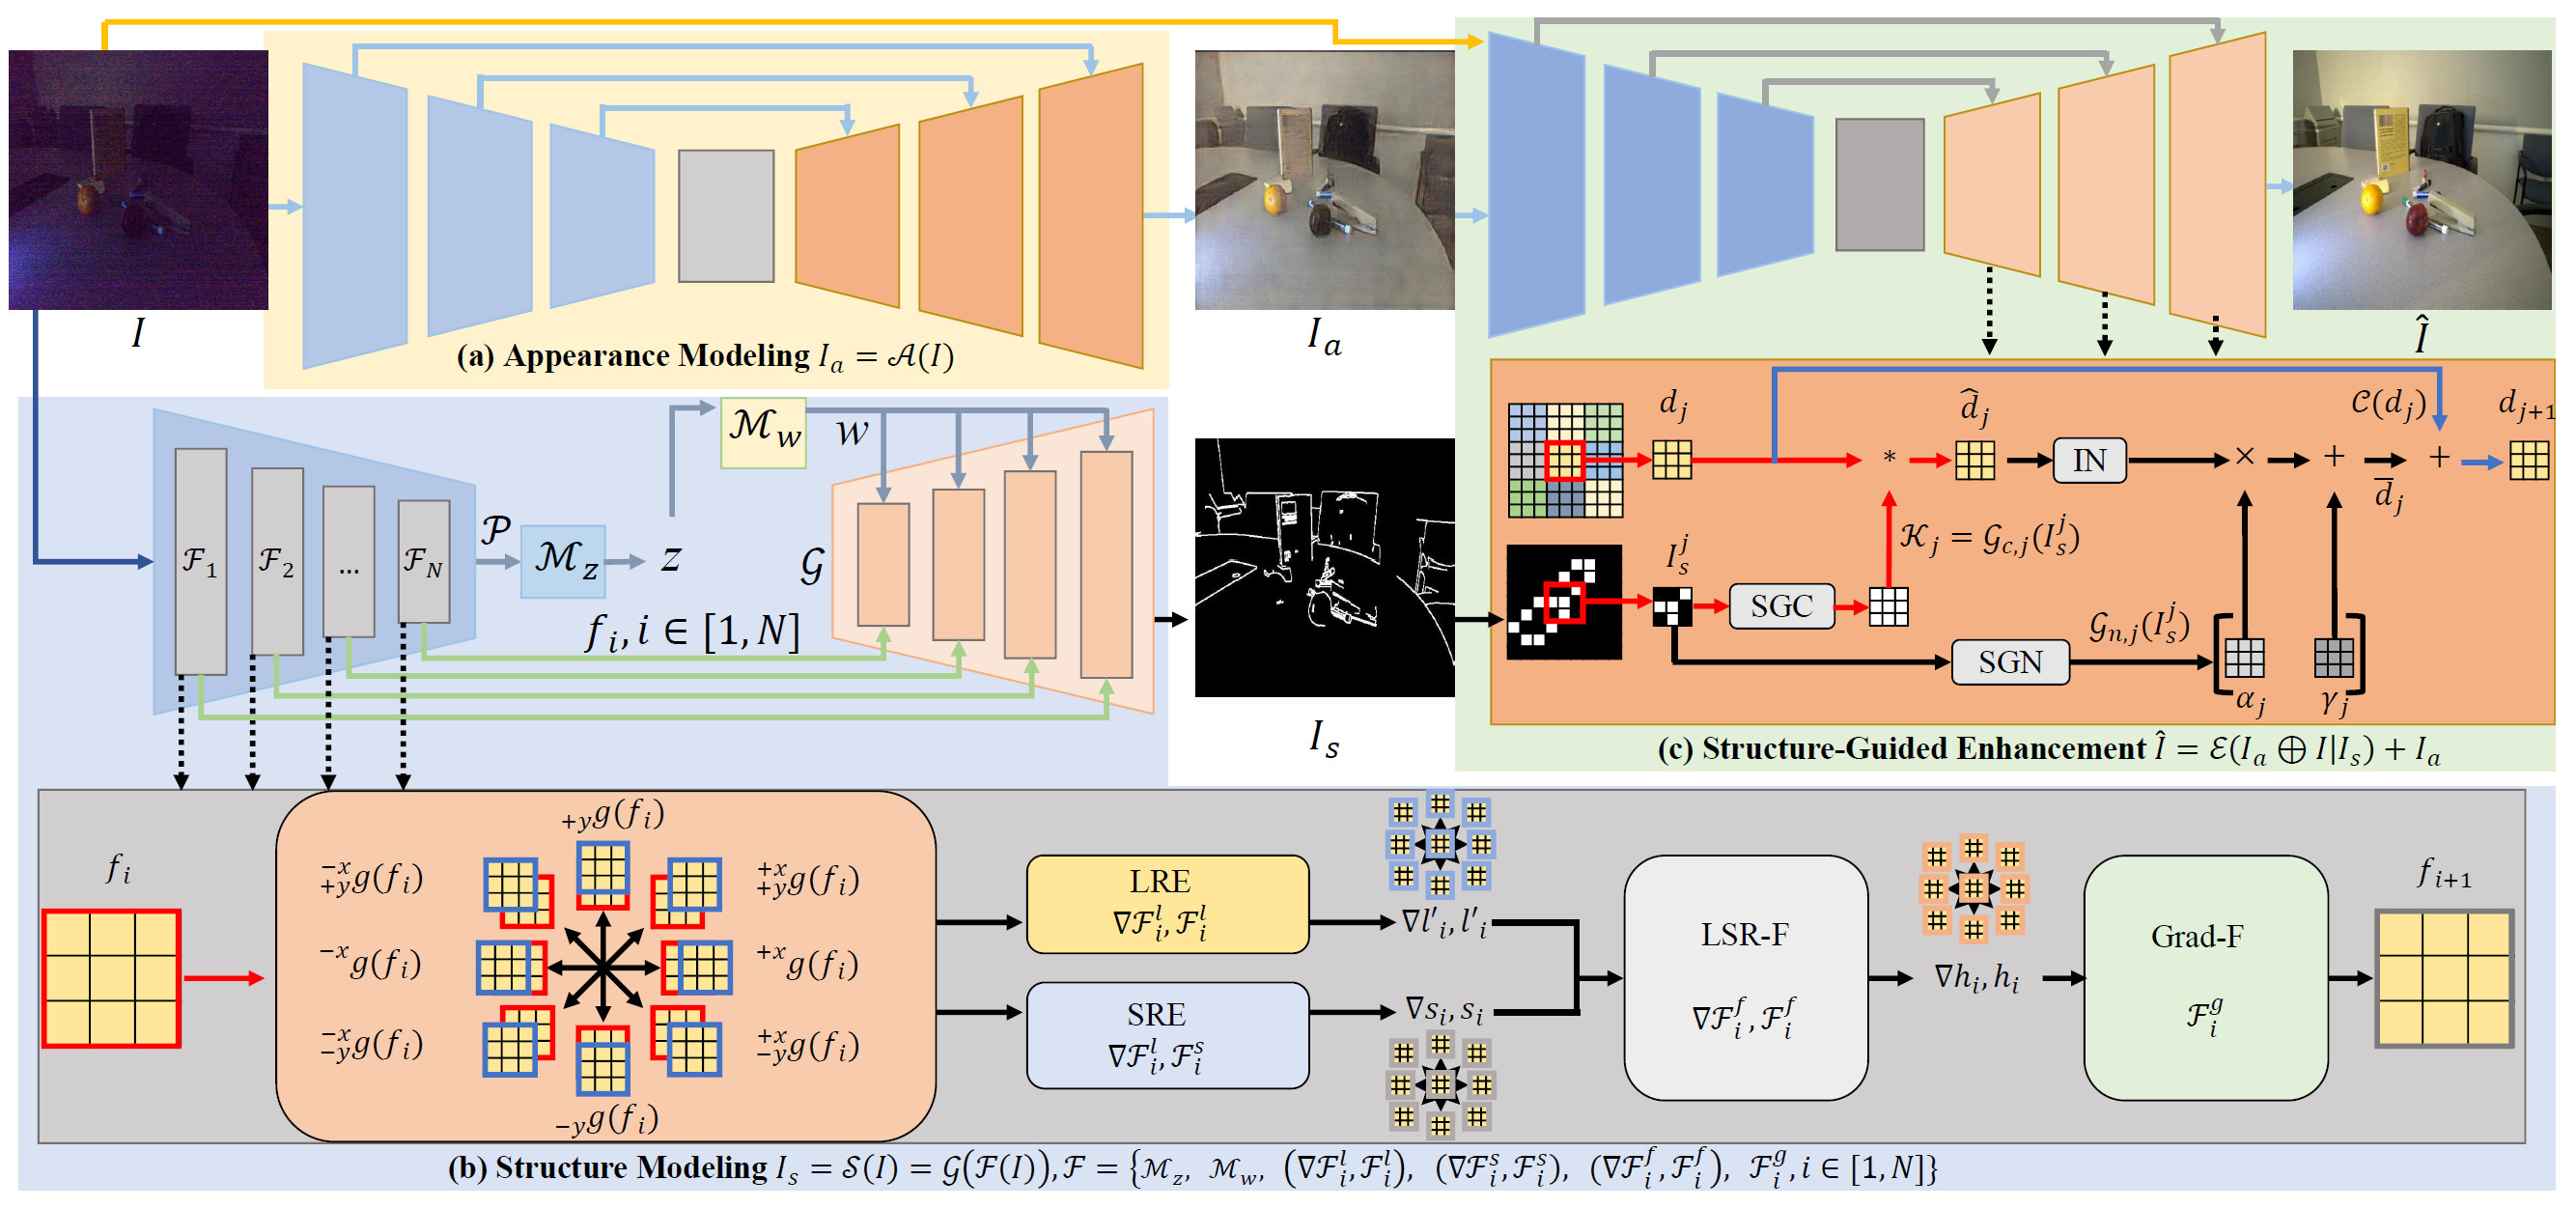
\includegraphics[width=0.8\textwidth]{picture/LLIE/Structure Modeling and Guidance/Overview}
			\end{center}
		\end{figure}
		
		\begin{minipage}{.45\textwidth}
			\textbf{\tiny Architecture}
			\begin{itemize}\tiny
			\item [-] U-Net
			% 通过一个简单的 U-Net 去对外观建模,可以理解成先简单地学习到一个正常光照的 coarse version。其中,损失函数为一个重建损失加感知损失。
					
			\item [-] Structure-Aware Feature Extractor
			% 对于结构信息建模部分,借鉴了 GAN prior 的思路,但是不用预训练的GAN 模型。这里设计到一个结构特征的提取Structure-Aware Feature Extractor (SAFE)
					
			\item [-] Structure-Guided Enhancement Module
			% 为了利用得到的结构图来提高外观,作者设计了一个结构导向增强模块 Structure-Guided Enhancement Module(SGEM模块)初始外观建模结果。在 SGEM 中,根据结构映射生成空间自适应核和归一化参数。然后,对SGEM 解码器的每一层的特征进行空间全处理y−自适应卷积和归一化。虽然 SGEM 的整体架构采用了一个简单的U-Net 的形式,但它可以有效地增强原始的外观。
			\end{itemize}
		\end{minipage}
		\begin{minipage}{.45\textwidth}
			\textbf{\tiny Edge Detection}
			\begin{itemize}\tiny
			\item [-] Too few datasets for extracting edge information
			% 论文指出低光数据集图片较少,所以结构信息提取模块的训练会受限,因此作者引入其他结构信息提取的数据集做额外训练可以进一步提升performance
			
			\item [-] Semantic maps and depth maps
			% 作者提出除了边缘结构图作为引导信息,也可以使用其他特征,比如语义图( Ours with SEG.)和深度图( Ours with Dep.),总体表现没有边缘图好,但是也比一些现有的增强方法好。
			
			\item [-] Input image or initial enhanced image
			% 作者没有说 Appearance Modeling 的结果去提取边缘会达到什么效果?
			
			% 此外作者做消融实验的过程中,使用一个 SOTA 边缘提取网络代替论文中的structural modeling 模块(但是感觉在低光照下很难提取到有效的边缘,合理点的话需要先对输入亮度增强一下)
			\end{itemize}
		\end{minipage}
	\end{frame}
	
	\subsection{Conformer}
	
	\begin{frame}
		Conformer: Local Features Coupling Global presentations for Visual Recognition\textcolor{blue}{\citep{peng2021conformer}}
		\begin{itemize}
			\item \textbf{Background}
			\item[\checkmark]
			Transformer is introduced into the visual task. 
			% Transformer 被引入视觉任务
			
			\item[\checkmark]
			Vision Transformer reflect the complex spatial transformations and long-distance feature dependence.
			% 由于自注意力机制和多层感知器 MLP 结构,Vision Transformer反映了复杂的空间变换和远距离特征依赖,它们构成了全局表示。
			
			\item[\checkmark]
			Local feature details are ignored.
			% Vision Transformer 反映了复杂的空间变换和远距离特征以来,他们构成了全局表示。
		\end{itemize}
		
		\begin{figure}[htbp]
			\begin{center}
				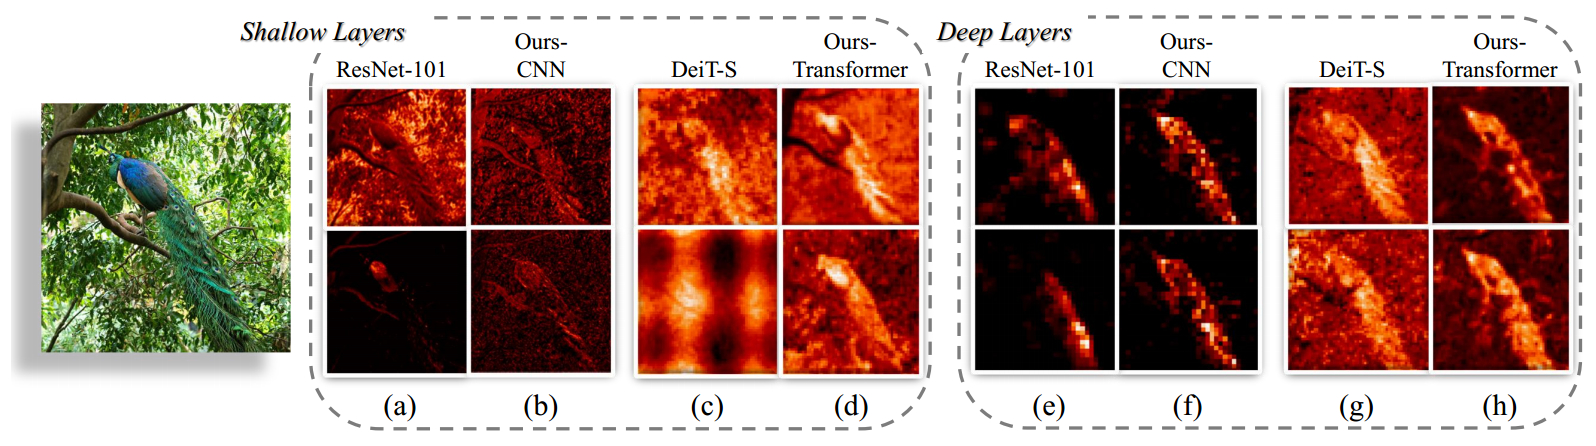
\includegraphics[width=0.8\textwidth]{picture/LLIE/Conformer/Comparison of feature maps of CNN (ResNet-101)}
			\end{center}
		\end{figure}
		
		% CNN (ResNet-101)、Visual Transformer (DeiT-S)和所提出的 Conformer 的特征图比较。变压器中的贴片嵌入被重塑为特征映射,以实现可视化。CNN 激活了判别性的局部区域(例如: 孔雀的头部(a)和尾部(e)), Conformer 的 CNN 分支利用了来自视觉变压器的全局线索,从而激活了完整的对象(例如: 孔雀的整个范围(b)和(f))。与 CNN 相比,视觉变压器的局部特征细节变差(例如: (c), (g))。Conformer的 Transformer 分支保留了 CNN 的局部特征细节,同时压制了背景(例如: (d)和(h)中的孔雀轮廓比(c)和(g)中的孔雀轮廓更完整)。(以彩色观看效果最佳)
	\end{frame}
	
	\begin{frame}
		
		
		\begin{figure}
			\centering
			\begin{minipage}{.4\textwidth}
				\centering
				\small
				\begin{itemize}
					\item \textbf{Contribution}
					
					\item[\checkmark]
					A Dual Network Structure
					% 一种双重网络结构
					
					\item[\checkmark]
					CNN and Transformer Branch
					% Conformer由 CNN 和 Transformer 分支组成,分别遵循 ResNet 和 ViT 的设计,这两个分支形成了 local convolution blocks,自注意力模块和 MLP 的组合。
					
					\item[\checkmark]
					Cross-entropy Loss Function
					% 在训练期间,使用交叉熵损失函数用于监督 CNN 和 Transformer 分支
					
					\item[\checkmark]
					Feature Coupling Unit (FCU)
					% 考虑到 CNN 和 Transformer 之间的特征错位(feature misalignment),特征耦合单元 Feature Coupling Unit(FCU) 被设计为 bridge,一方面为了融合这两种风格特征,FCU 利用 1x1 卷积来对齐通道尺寸,利用向上/向下采样策略来对齐分辨率,利用LN,BN对齐特征值。
				\end{itemize}
				\captionsetup{font=scriptsize}
				\label{fig: Contribution}
				%\caption*{Contribution}
			\end{minipage}
			\begin{minipage}{.58\textwidth}
				\centering
				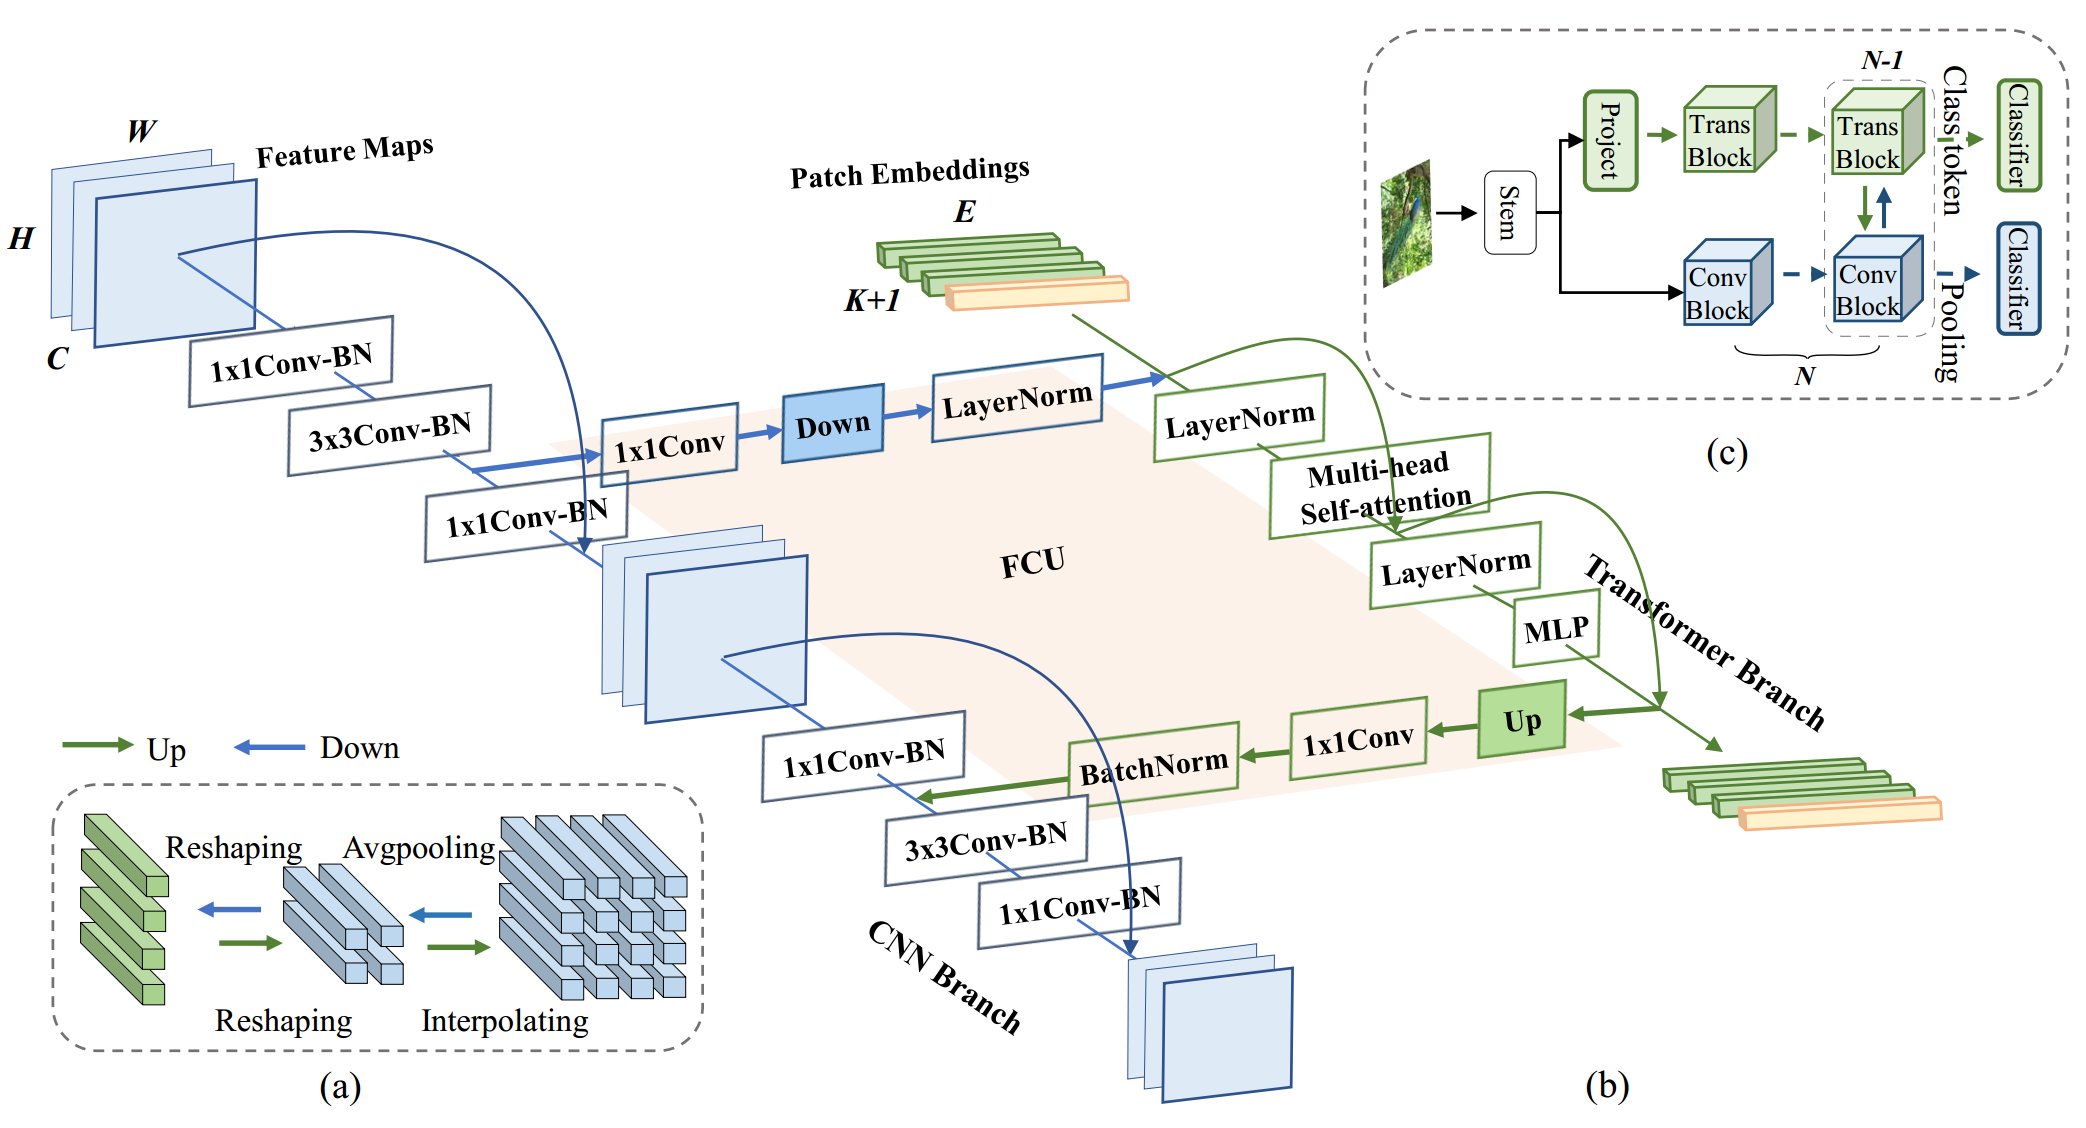
\includegraphics[width=\linewidth]{picture/LLIE/Conformer/the proposed Conformer}
				\captionsetup{font=scriptsize}
				\label{fig: Conformer}	
				\caption*{Conformer}
			\end{minipage}
			\captionsetup{font=scriptsize}
			\caption{
				\label{fig: Conformer contribution}
				Network architecture of the proposed Conformer.
			}
		\end{figure}
		
	\end{frame}
	
	\section{Proposed Model}
	
	\subsection{Total Architecture}
	
	\begin{frame}
		
		Our study focuses on constructing an overall recovery framework that utilizes the fusion of edge maps, preliminary recovery maps, and channel information to improve the quality of low-light images.
		
		% 我们的研究侧重于构建一个整体恢复框架,该框架利用边缘图、初步恢复图和通道信息的融合,以提高弱光图像的质量。我们将继续探索合适的增强网络结构,以便进一步提升恢复结果的性能。这一研究旨在为弱光图像恢复领域提供新的理论和方法,以及改善图像质量并拓展应用领域。
		
		\begin{itemize} 
			\item \textbf{Model for the initial recovery }
			% 初步恢复的模型
			
			\small Drawing on the conformer parallel structure, CNN branched Res-Net structure is modified to the U-Net structure.
			% 我们受到了 Conformer 结构的启发,在卷积神经网络 (CNN) 中,卷积操作擅长提取局部特征,但难以捕获全局表示。Conformer 是一种混合网络结构,包含了混合网络结构,包含了并行的 CNN 分支和 Transformer 分支,其通过特征耦合模块融合局部与全局特征,目的在于不损失图像细节的同时捕捉图像全局信息。我们借鉴 Conformer 并发结构,将其中 CNN 分支的 ResNet 结构修改为 U-Net 结构。基于这一点,我们设计了一种结合U-Net 与Transformer 网络的并行模型(PACUT, Parallel architecture combining u-net and transformer)。这一模型旨在从弱光图像中提取长距离和短距离特征,以便更全面地捕捉图像的信息。通过特定的特征融合策略,我们期望能够得到初步恢复的图像。

			\item \textbf{Low-light image edge generation network}
			% 弱光图像边缘生成网络
			
			\small Multi-exposure Architecture
			% 多曝光架构
			
			\small HOG and LBP guided
			% HOG 和 LBP 融合
			
			
			\item \textbf{Edge-guided enhancement}
			% 边缘图像指导恢复网络
			
			\small Series fusion
			% 串联融合
			
			\item \textbf{Challenge}
			
			\small The coordination of the overall model
			% 整体模型的协调性
			
			\small Ablation Study
			% 消融实验
			
			
		\end{itemize}
		
	\end{frame}
	
	\begin{frame}
		
		\begin{figure}[htbp]
			\begin{center}
				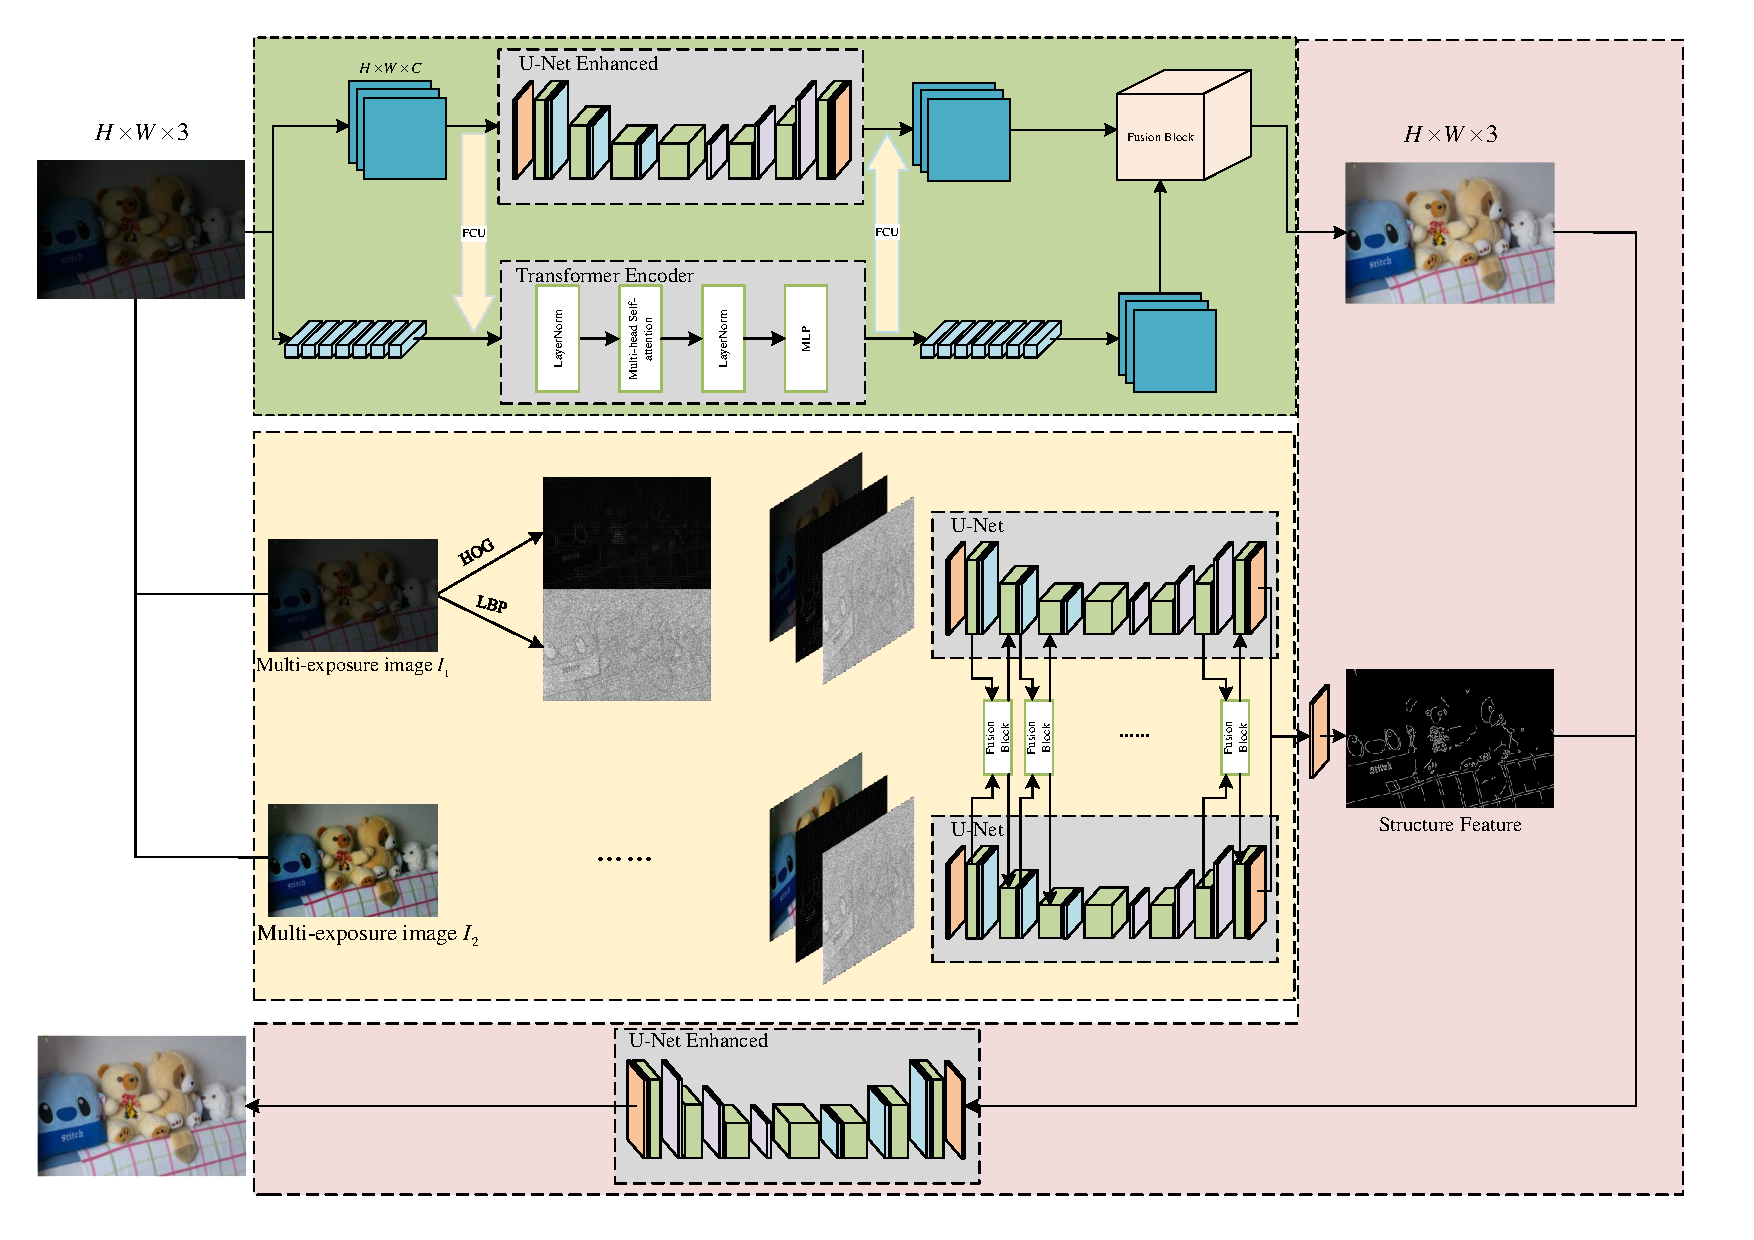
\includegraphics[width=0.65\textwidth]{picture/LLIE/My Architecture/Total architecture}
			\end{center}
			\captionsetup{font=scriptsize}
			\caption{
				\label{fig: Total architecture}
				Total Architecture
			}
		\end{figure}
		
	\end{frame}
	
	\subsection{PACUT}
	
	\begin{frame}
		\begin{figure}
			\centering
			\begin{minipage}{.4\textwidth}
				\centering
				\small
				% 在当前的研究中,我们提出了一种新型的深度学习架构,命名为 PACUT ,旨在解决低光照条件下的图像增强问题。该模型结合了经典的 U-Net 架构和 Transformer 深度学习方法,在弱光图像增强任务中,提高恢复图像的可视性和质量,同时保留重要的细节和纹理信息。此分支的设计旨在处理图像的低级特征,如边缘、纹理和颜色信息。
				\begin{itemize} 
					\item \textbf{Abstract}
					
					\item[\checkmark]\small Based Conformer
					
					\item[\checkmark]\small Long-and short-distance feature
					
				\end{itemize}
				\begin{itemize} 
					\item \textbf{Key improvements}
					
					\item[\checkmark]\small CNN Branch
					
					% 深度卷积网络(CNN)分支:该分支基于 U-Net 架构,采用多层卷积神经网络,通过逐层提取图像的局部特征来增强图像的细节和纹理。
					
					\item[\checkmark]\small Feature Coupling Unit
					
					% 特征耦合单元(FCU):为了有效地融合 CNN 分支和 ViT 分支的特征,引入了特征耦合单元(FCU)。FCU 通过下采样(FCUDown) 和上采样(FCUUp) 操作,实现了CNN特征图和Transformer patch embeddings 之间的无缝转换,从而实现了局部特征和全局表示的连续耦合。
				\end{itemize}
				\captionsetup{font=scriptsize}
				\label{fig: Abstract}
				%\caption*{Contribution}
			\end{minipage}
			\begin{minipage}{.58\textwidth}
				\centering
				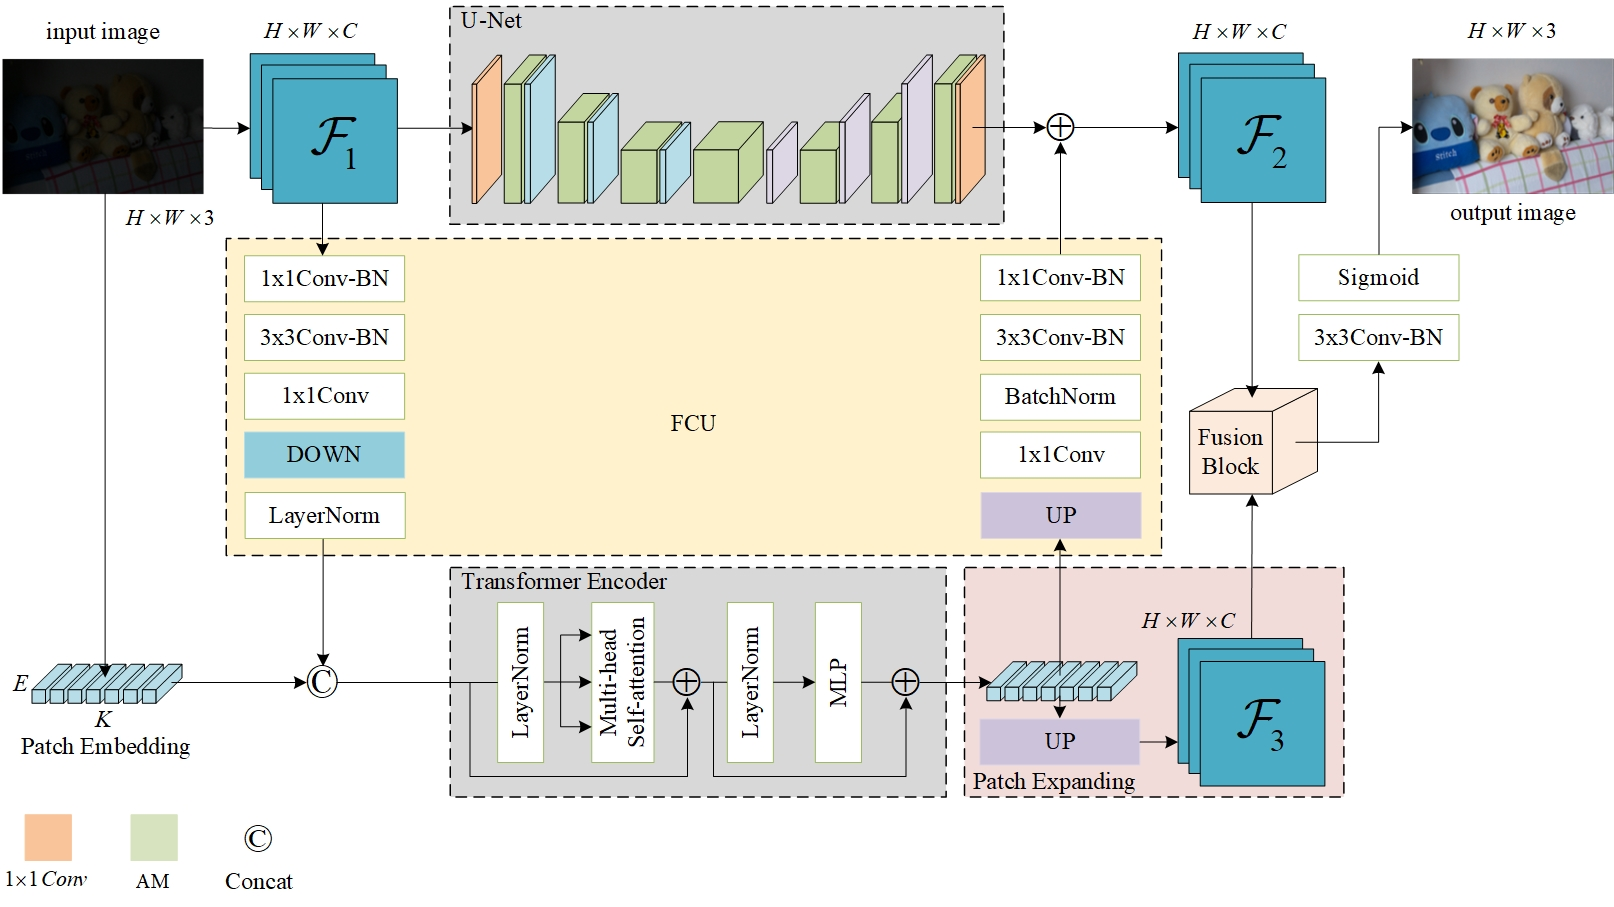
\includegraphics[width=.88\linewidth]{picture/LLIE/My Architecture/The proposed initial architecture.jpg}
				\captionsetup{font=scriptsize}
				\label{fig: PACUT}	
				\caption*{\tiny PACUT}
			\end{minipage}\\
			\hfill
			\begin{minipage}{.28\textwidth}
				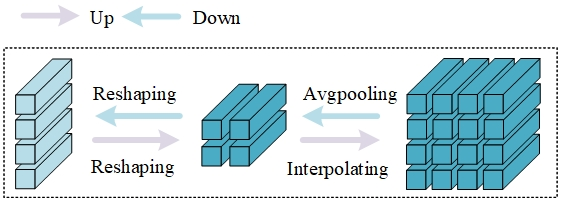
\includegraphics[width=.88\linewidth]{picture/LLIE/My Architecture/Up-sampling and down-sampling.jpg}
				\captionsetup{font=scriptsize}
				\label{fig: Up-sampling and down-sampling}	
				\caption*{\tiny Up-sampling and down-sampling}
			\end{minipage}
			\begin{minipage}{.28\textwidth}
				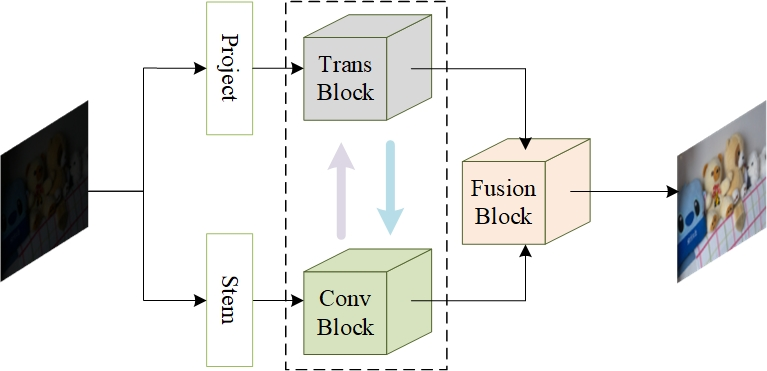
\includegraphics[width=.88\linewidth]{picture/LLIE/My Architecture/The proposed initial architecture(Abstract Picture).jpg}
				\captionsetup{font=scriptsize}
				\label{fig: The proposed initial architecture(Abstract Picture)}	
				\caption*{\tiny Thumbnail of PACUT}
			\end{minipage}
			\captionsetup{font=scriptsize}
			\caption{
				\label{fig: Parallel architecture combining u-net and transformer}
			}
		\end{figure}
		
	\end{frame}
	
	\begin{frame}
		
		\begin{itemize} 
			\item \textbf{CNN Branch}
			
			\small The foundation of the CNN branch is the U-Net structure, a network architecture designed specifically for image segmentation tasks, but also outstanding in the field of image enhancement.
			% CNN 分支的基础是 U-Net 结构,这是一种专门为图像分割任务设计的网络架构,但在图像增强领域也表现出色。U-Net 的特点是其对称的编码器-解码器结构,以及编码器和解码器之间的跳跃连接。CNN 分支的目标是从输入的弱光图像(LLI) 中提取丰富的特征,包括边缘、纹理、颜色、亮度信息,并最终输出增强的图像(EI)。
			
			\checkmark \small UNetEnhanced Method
			% UNetEnhanced 模型是一种针对低光照图像增强任务设计的深度学习架构。该模型基于经典的U-Net 架构,并引入了多项改进,以提高对低光照环境下图像的处理能力。这些改进包括更深的网络结构、改进的特征融合机制和高效的信息传递路径。
		\end{itemize}
		
		% UNetEnhance 模型由两个部分组成:1) 编码器子网络(Encoder subnetworker),2) 解码器子网络(Decoder subnetworker)。对于编码器子网络,UNetEnhance 采用了多层卷积网络,在每层中我们添加了集成模块,在集成模块中又添加了空间注意力机制和通道注意力机制。与传统 U-Net 相比,这一设计增加了网络的深度,从而能够捕获更加丰富的特征信息。我们通过引入更多的卷积层,使得模型能够在更深的层次上理解图像内容。解码器部分采用了上采样和卷积操作,以逐步恢复图像的空间分辨率。
		
		% 在这一过程中,引入了改进的特征融合策略,将编码器中的低级特征与解码器的高级特征有效结合,从而更好地重建图像细节。同时,UNetEnhance 模型在跳跃连接的设计上进行了优化,以更有效地传递编码器中的特征信息到编码器。这些连接不仅帮助保留了在下采样过程中可能丢失的细节信息,还增强了网络的特征重建能力。此外,模型的输出层经过特别设计,以确保输出图像在视觉上的质量和连贯性,我们通过准确的调整解码器子网络中的卷积操作,将解码器的输出转换为与原始输入图像相同尺寸的增强图像。
		
		\begin{figure}
			\centering
			\begin{minipage}{.65\textwidth}
				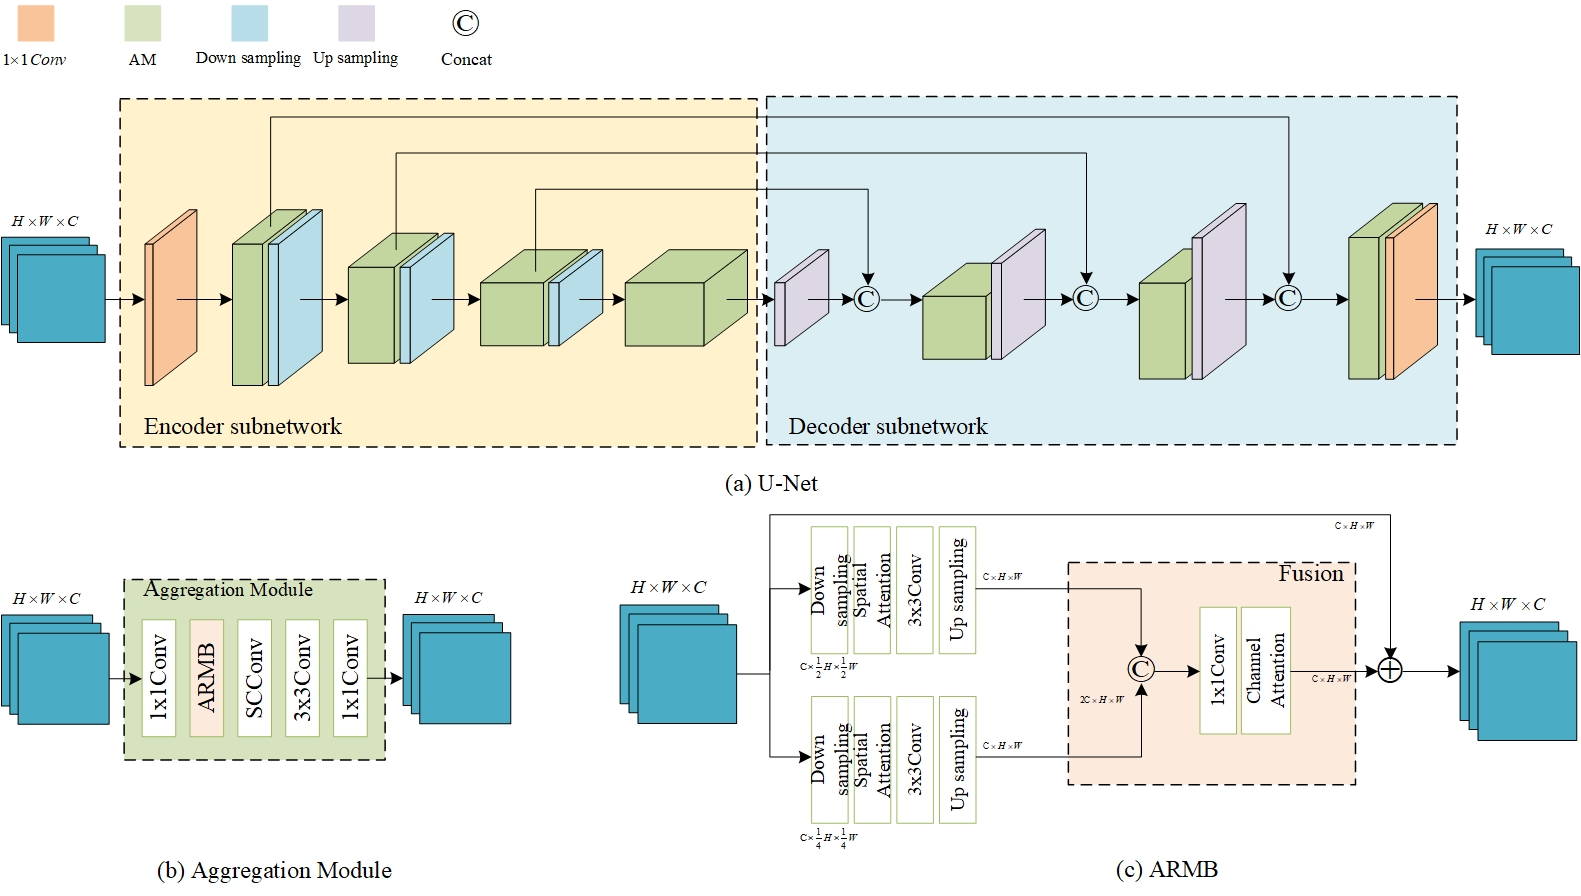
\includegraphics[width=0.85\linewidth]{picture/LLIE/My Architecture/U-Net and AM.jpg}
				\captionsetup{font=scriptsize}
				\label{fig: U-Net and AM}	
				\caption*{UNetEnhanced Method}
			\end{minipage}
			\captionsetup{font=scriptsize}
			\caption{
				\label{fig: CNN Branch}
			}
		\end{figure}
		
	\end{frame}
	
	\begin{frame}	
		
		Assuming that $I_{LLI}$ represents the input low-light image and $I_{EI}$ represents the enhanced image of the output. The operation of the encoder subnetwork $\mathcal{E}$ and the decoder subnetwork $\mathcal{D}$ can be expressed as:
		% 假设ILLI 表示输入的弱光图像,IEI 表示输出的增强图像。编码器子网络 E 和解码器子网络 D 的操作可以表示为:
		\begin{block}{UNetEnhanced}
			\begin{equation}
				\begin{aligned}
					I_{EI} = \mathcal{D} \left( \mathcal{E} \left( I_{LLI} \right) \right)
				\end{aligned}
				\label{eq: UNetEnhance model}
			\end{equation}
		\end{block}
		
		\begin{block}{Aggregation Module}
			\begin{equation}
				\begin{aligned}
					\text{AM}_{i}(x) = f^{1 \times 1} \left(f^{3 \times 3} \left(\text{SCConv}\left( \text{ARMB} \left( f^{1 \times 1} (x)\right)\right)\right)\right)
				\end{aligned}
			\end{equation}
		\end{block}
		
		Where $f ^ {1 \times 1} $ is the $1 \times 1$ convolution layer, and the operation of ARMB and SCConv depends on their internal structure.
		% 其中,f1×1为1 × 1 卷积层,ARMB 和SCConv 的操作依据其内部结构进行。
	\end{frame}
	
	\begin{frame}	
		
		ARMB (Attention Residual Merging Block) 
		
		% ARMB (Attention Residual Merging Block) 是一种用于深度学习模型中的结构单元,特别是在处理图像相关任务时,它的主要作用是融合来自不同来源的特征,并通过注意力机制增强模型对关键信息的关注。其核心作用之一是融合来自模型不同层或不同分支的特征。
		
		Suppose $ \mathcal {F} _ {in} $ is the input feature graph, $ \mathcal {F} _ {out} $ is the output feature graph, $ \mathcal {F} _ {i} ^ \prime$ means that the feature graph is trimmed or enlarged, see the following equation:
		
		% 假设Fin 是输入特征图,Fout 是输出特征图,F′i 表示对特征图进行裁剪或放大,见下式:
		
		\begin{block}{ARMB}
			\begin{equation}
				\begin{aligned}
					&\mathcal{F}^\prime_{\frac{1}{2}} = \text{Resize}\left(\mathcal{F}_{in},\left(\frac{H}{2},\frac{W}{2}\right)\right), \\
					&\mathcal{F}^\prime_{\frac{1}{4}} = \text{Resize}\left(\mathcal{F}_{in},\left(\frac{H}{4},\frac{W}{4}\right)\right), \\
					&\mathcal{F}_{out} = W_1\mathcal{F}_{out} + W_2\mathcal{C} \left( f^{1 \times 1}  \left[\mathcal{F}^\prime_2 (f^{3 \times 3}(\mathcal{S}(\mathcal{F}^\prime_{\frac{1}{2}}))), \mathcal{F}^\prime_4 (f^{3 \times 3}(\mathcal{S}(\mathcal{F}^\prime_{\frac{1}{4}})))\right] \right).
				\end{aligned}
				\label{eq: ARMB}
			\end{equation}
		\end{block}
		
		Where $ \mathcal{S} $ and $ \mathcal{C} $ represent the spatial and channel attention function, respectively, and $W_1$ and $W_2$ are the corresponding feature graph weights.
		
		% 其中S 和 C 分别表示空间注意力函数和通道注意力函数,W1 和W2 为对应的特征图权重。
	\end{frame}
	
	\begin{frame}
		\begin{figure}
			\centering
			\begin{minipage}{.45\textwidth}
			\begin{itemize} 
				\item \textbf{Transformer Branch}
				
				Based Vision Transformer (ViT)
				
				Extract global features
				% 这一分支的目标是捕获图像中的长距离依赖关系,以辅助CNN 分支的局部特征提取。
				
			\end{itemize}
			
	
			\begin{itemize} 
				\item \textbf{Patch Embedding}
				% Patch Embedding是一种常见的操作,它将图像分割成更小的块(patches),然后将这些块转换成一系列的向量,这些向量可以被用作模型的输入。
				
				\item[\checkmark] Segmenting
				
				\item[\checkmark] Reshape
				
				\item[\checkmark] Flatten
				
				\item[\checkmark] Linear Projection
				
			\end{itemize}
			\end{minipage}
			\begin{minipage}{.45\textwidth}
				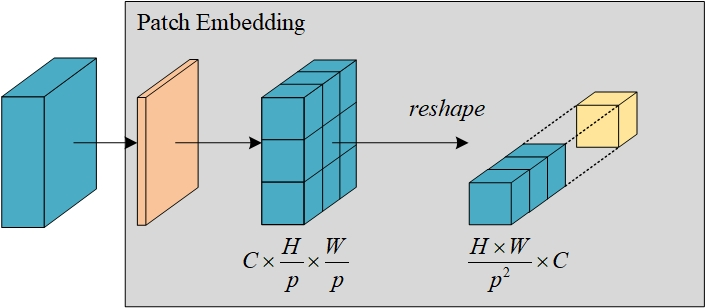
\includegraphics[width=0.85\linewidth]{picture/LLIE/My Architecture/Patch Embedding}
				\captionsetup{font=scriptsize}
				\caption*{Patch Embedding}
			\end{minipage}
			\captionsetup{font=scriptsize}
			\caption*{
				\label{fig: Patch Embedding}
			}
		\end{figure}
	\end{frame}

	\begin{frame}
		\begin{figure}
			\centering
			\begin{minipage}{.95\textwidth}
				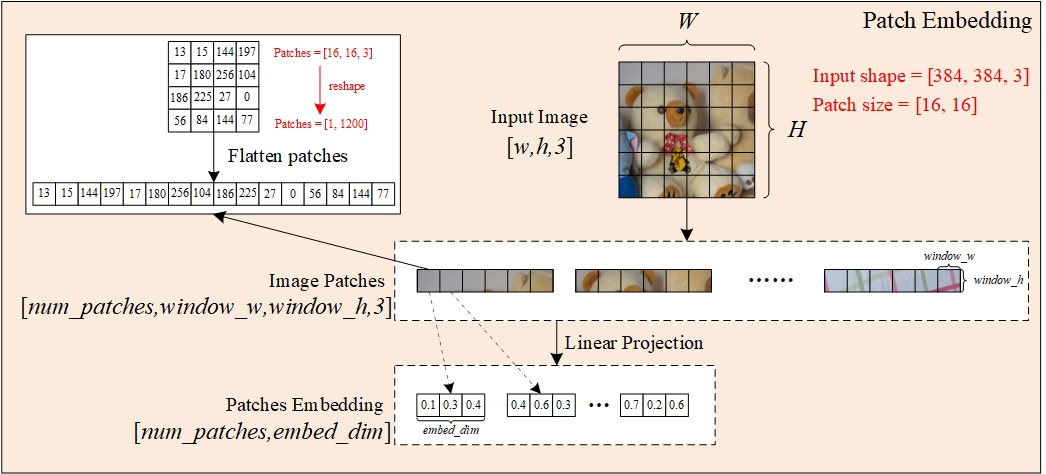
\includegraphics[width=\linewidth]{picture/LLIE/My Architecture/Patch Embedding(ViT)}
				\captionsetup{font=scriptsize}
				\caption{Patch Embedding in Transformer Branch}
			\end{minipage}
			\captionsetup{font=scriptsize}
			\caption*{
				\label{fig: Patch Embedding in ViT}
			}
		\end{figure}
	\end{frame}
	
	\begin{frame}
		\begin{itemize} 
			\item \textbf{Feature Coupling Unit}
			% CNN 分支中特征映射和Transformer 分支中patch embedding,如何消除他们之间的错误是一个重要的问题,为了解决这个问题,使用FCU 以交互的方式将局部特征和全局表示进行连续耦合。
			
			Feature mapping in CNN branch and patch embedding in Transformer branch, how to eliminate errors between them is an important question, and to solve this problem, the FCU is used to continuously couple local features and global representations in an interactive manner.
			
			\item[\checkmark] CNN dim: $H \times W \times C$
			
			\item[\checkmark] Transformer dim: $K \times D$
			% 其中K, D分别表示图像 patch 的数量和 embedding 的维度。用于分类的 Vision Transformer 模型中 patch embedding 的形状为 (K + 1)×D,其中 1 为类别嵌入 (Class Token),但是在 Transformer 分支中,我们去除了类别嵌入。			
			
			% 特征映射和patch embedding 之间存在显著的语义鸿沟,即特征映射是从局部卷积算子收集的,而 patch embedding 则是通过自注意力机制聚合的,所以通过应用 FCU 可以填补语义空白。 
		\end{itemize}
	\end{frame}
	
	\subsection{Edge Detection Network}
	
	\begin{frame}
		
		\begin{itemize} 
			\item \textbf{Traditional Method}
			% 获取图像边缘的深度学习方法主要依赖于卷积神经网络(CNN)的变体和架构,这些方法能够有效地提取图像的特征,包括边缘信息。以下是一些常见的深度学习方法,用于获取图像边缘。
			
			CNN
			% 传统的CNN架构,如LeNet、AlexNet、VGGNet等,可以通过训练来识别图像边缘。在这些网络的初级层中,通常会学习到类似于传统边缘检测滤波器(如 Sobel 或 Canny)的特征。
			
			Auto-encoder
			% 自编码器可以用于学习图像的压缩表示,其中编码器部分可以被训练来提取图像的边缘信息。
			
			GANS
			% GANs可以用于边缘检测,特别是在图像到图像的转换任务中
			
			U-Net
			% U-Net是一种流行的用于图像分割的网络架构,它也可以被用于边缘检测。U-Net的对称结构和跳跃连接特别适合于捕捉图像的细节和边缘。
		\end{itemize}
		\begin{itemize} 
			\item \textbf{Challenge}
			
			Processing dark light images directly can distort the edge map
			% 直接处理暗光图片会使得边缘图失真
			
		\end{itemize}
	\end{frame}
	
	\begin{frame}
		\begin{figure}
			\centering
			\begin{minipage}{.19\textwidth}
				\centering
				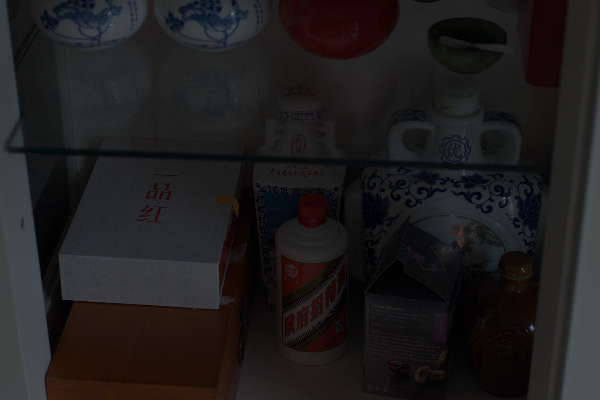
\includegraphics[width=.8\linewidth]{picture/LLIE/My Architecture/Edge Detection/low00044}
				\captionsetup{font=scriptsize}
				\label{fig: LLI}
				\caption*{LLI}
			\end{minipage}
			\begin{minipage}{.19\textwidth}
				\centering
				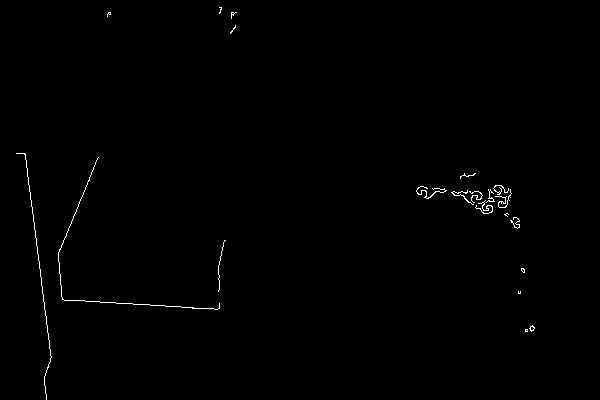
\includegraphics[width=.8\linewidth]{picture/LLIE/My Architecture/Edge Detection/low00044_canny}
				\captionsetup{font=scriptsize}
				\label{fig: LLI_canny}	
				\caption*{LLI Canny}
			\end{minipage}
			\begin{minipage}{.19\textwidth}
				\centering
				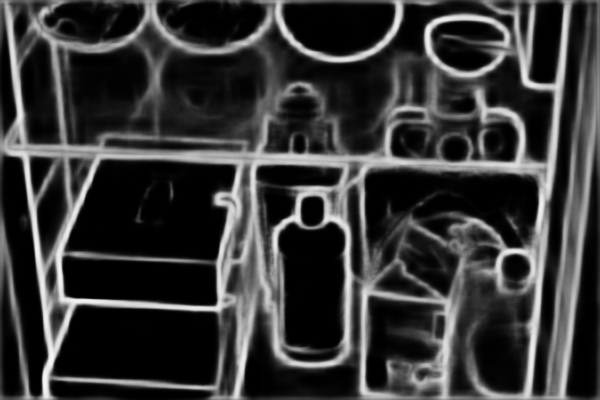
\includegraphics[width=.8\linewidth]{picture/LLIE/My Architecture/Edge Detection/low00044_rcf}
				\captionsetup{font=scriptsize}
				\label{fig: LLI_rcf}	
				\caption*{LLI RCF}
			\end{minipage}
			\begin{minipage}{.19\textwidth}
				\centering
				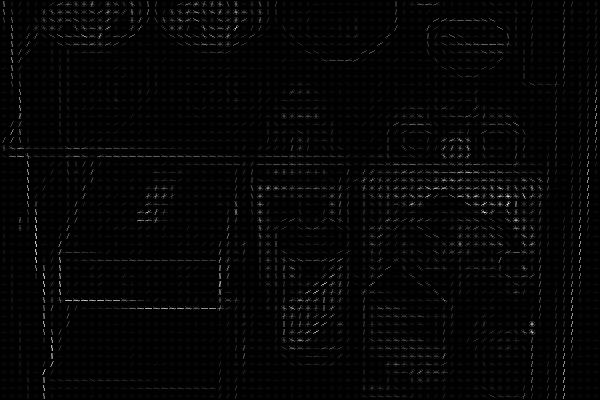
\includegraphics[width=.8\linewidth]{picture/LLIE/My Architecture/Edge Detection/low00044_hog}
				\captionsetup{font=scriptsize}
				\label{fig: LLI_hog}	
				\caption*{LLI HOG}
			\end{minipage}
			\begin{minipage}{.19\textwidth}
				\centering
				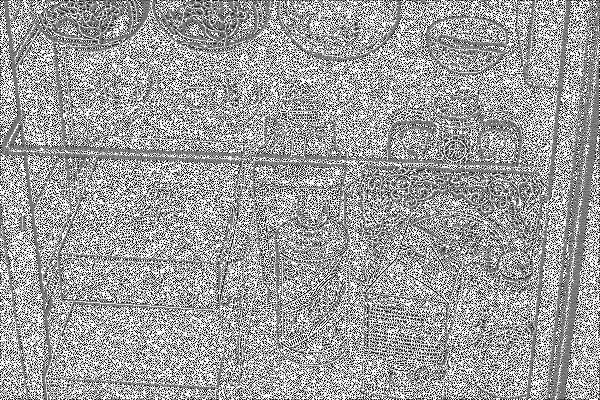
\includegraphics[width=.8\linewidth]{picture/LLIE/My Architecture/Edge Detection/low00044_lbp}
				\captionsetup{font=scriptsize}
				\label{fig: LLI_lbp}	
				\caption*{LLI LBP}
			\end{minipage}
			\begin{minipage}{.19\textwidth}
				\centering
				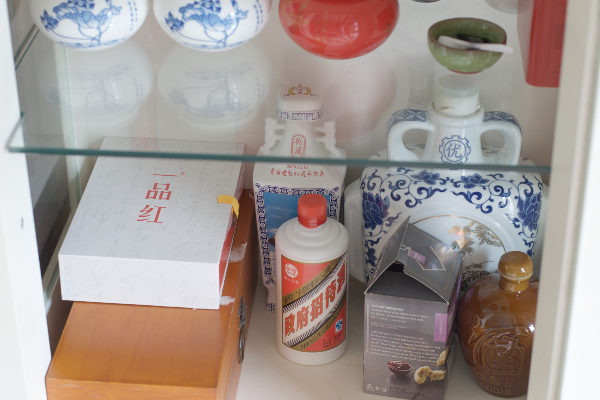
\includegraphics[width=.8\linewidth]{picture/LLIE/My Architecture/Edge Detection/normal00044}
				\captionsetup{font=scriptsize}
				\label{fig: GI}
				\caption*{GT}
			\end{minipage}
			\begin{minipage}{.19\textwidth}
				\centering
				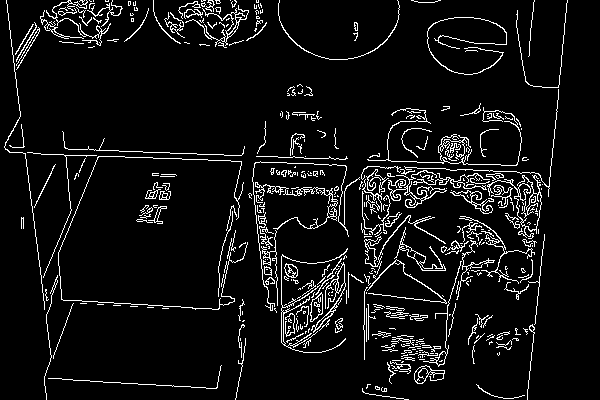
\includegraphics[width=.8\linewidth]{picture/LLIE/My Architecture/Edge Detection/normal00044_canny}
				\captionsetup{font=scriptsize}
				\label{fig: GT_canny}	
				\caption*{GT Canny}
			\end{minipage}
			\begin{minipage}{.19\textwidth}
				\centering
				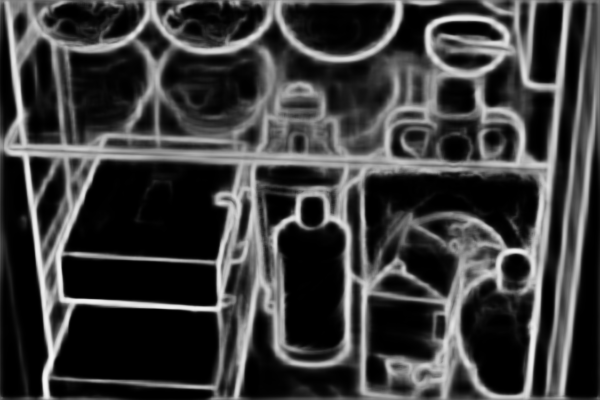
\includegraphics[width=.8\linewidth]{picture/LLIE/My Architecture/Edge Detection/normal00044_rcf}
				\captionsetup{font=scriptsize}
				\label{fig: GT_rcf}	
				\caption*{GT RCF}
			\end{minipage}
			\begin{minipage}{.19\textwidth}
				\centering
				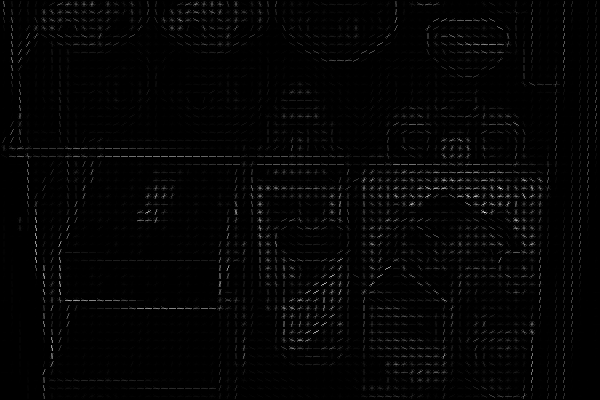
\includegraphics[width=.8\linewidth]{picture/LLIE/My Architecture/Edge Detection/normal00044_hog}
				\captionsetup{font=scriptsize}
				\label{fig: GT_hog}	
				\caption*{GT HOG}
			\end{minipage}
			\begin{minipage}{.19\textwidth}
				\centering
				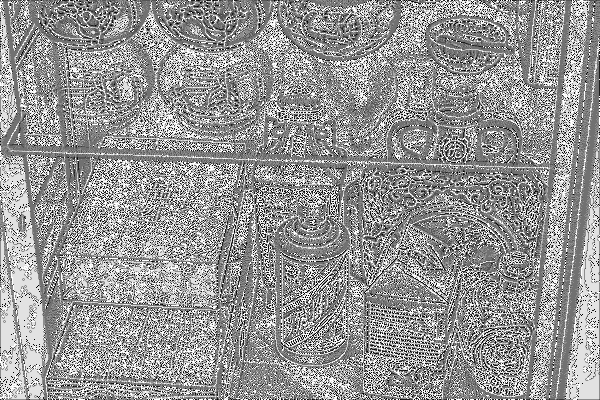
\includegraphics[width=.8\linewidth]{picture/LLIE/My Architecture/Edge Detection/normal00044_lbp}
				\captionsetup{font=scriptsize}
				\label{fig: GT_lbp}	
				\caption*{GT LBP}
			\end{minipage}
			\captionsetup{font=scriptsize}
			\caption{
				\label{fig: LLI Structure Information}
				LLI and GT Structure Information
			}
		\end{figure}
	\end{frame}
	
	\begin{frame}
		
		\begin{itemize} 
			\item \textbf{Histogram of Oriented Gradients, HOG}
			\vspace{.3cm}
			% 一般而言,HOG特征在物体检测(特别是行人检测)中非常有效,它通常与支持向量机(SVM)分类器一起使用。
			% HOG 主要原理是计算图像的梯度幅值和方向。具体来说先把图像分割个小的连续区域(Cell),计算每一个区域梯度方向的直方图,最后合并成更大的区域(Block) 来对直方图进行归一化,然后合并所有 Block 形成最终的 HOG 特征图。		
			
			\small HOG is a feature control for shape information and texture information for local images.
			% HOG 是一个用于局部图像的形状信息和纹理信息的特征控件。它基于图像的梯度方向来构建直方图。
			
			\small Vectors of the shape and edge information of the object in the image
			% HOG特征表示包含图像中对象的形状和边缘信息的向量,它分析了图像中局部梯度方向的分布。
			
			\small HOG maintains good invariance to both image geometry and optical deformation.
			% 由于HOG是在图像的局部方格单元上操作,所以它对图像几何的和光学的形变都能保持很好的不变性。
		\end{itemize}
		
		\begin{itemize} 
			\item \textbf{Local Binary Pattern, LBP}
			\vspace{.3cm}
			% 一般而言,HOG特征在物体检测(特别是行人检测)中非常有效,它通常与支持向量机(SVM)分类器一起使用。
			% HOG 主要原理是计算图像的梯度幅值和方向。具体来说先把图像分割个小的连续区域(Cell),计算每一个区域梯度方向的直方图,最后合并成更大的区域(Block) 来对直方图进行归一化,然后合并所有 Block 形成最终的 HOG 特征图。		
			
			\small LBP is an operator used to describe the local features of images
			% LBP 是一种用来描述图像局部特征的算子。
			
			\small LBP features have significant advantages such as gray invariance and rotation invariance.
			% LBP特征具有灰度不变性和旋转不变性等显著优点
			
			\small HOG maintains good invariance to both image geometry and optical deformation.
			% LBP主要工作原理如下:对于图像中的每个像素,考虑其周围的一个领域(例如,3 × 3 的窗口),然后将邻域中的每个像素与中心像素进行比较。如果领域像素的值大于或等于中心像素的值,则将其标记为1,否则标记为0。这样相邻的所有域都会产生一个二进制模式(例如,11100101),通过计算所有二进制模式的直方图作为图像的 LBP 特征。
		\end{itemize}
		
		\begin{itemize} 
			\item \textbf{What we can find from HOG and LBP?}
			\vspace{.3cm}
			
			\small Edge information
			
			\small Necessarily Work?
			% 是否一定有效?
			
			\small How to solve?
			
		\end{itemize}
	\end{frame}
	
	\begin{frame}
		\begin{figure}
			\centering
			\begin{minipage}{.32\textwidth}
				\centering
				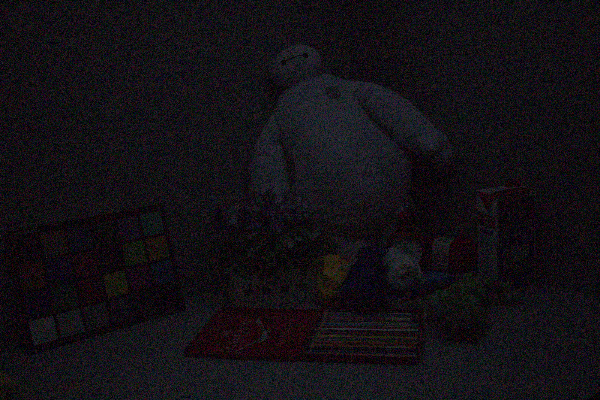
\includegraphics[width=.8\linewidth]{picture/LLIE/My Architecture/Edge Detection/low00269}
				\captionsetup{font=scriptsize}
				\label{fig: LLI1}
				\caption*{LLI with noise}
			\end{minipage}
			\begin{minipage}{.32\textwidth}
				\centering
				
\includegraphics[width=.8\linewidth]{picture/LLIE/My Architecture/Edge Detection/low00269_hog}
				\captionsetup{font=scriptsize}
				\label{fig: LLI_hog1}	
				\caption*{LLI HOG}
			\end{minipage}
			\begin{minipage}{.32\textwidth}
				\centering
				
\includegraphics[width=.8\linewidth]{picture/LLIE/My Architecture/Edge Detection/low00269_lbp}
				\captionsetup{font=scriptsize}
				\label{fig: LLI_lbp1}	
				\caption*{LLI LBP}
			\end{minipage}
			\begin{minipage}{.32\textwidth}
				\centering
				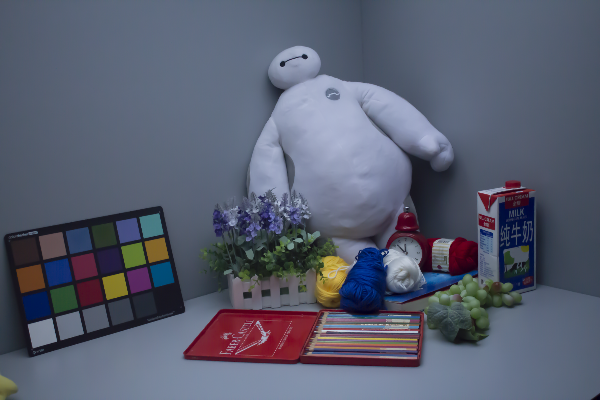
\includegraphics[width=.8\linewidth]{picture/LLIE/My Architecture/Edge Detection/normal00269}
				\captionsetup{font=scriptsize}
				\label{fig: GI1}
				\caption*{GT}
			\end{minipage}
			\begin{minipage}{.32\textwidth}
				\centering
				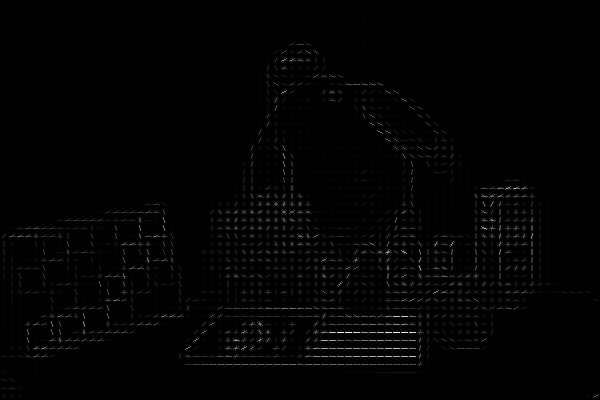
\includegraphics[width=.8\linewidth]{picture/LLIE/My Architecture/Edge Detection/normal00269_hog}
				\captionsetup{font=scriptsize}
				\label{fig: GT_hog1}	
				\caption*{GT HOG}
			\end{minipage}
			\begin{minipage}{.32\textwidth}
				\centering
				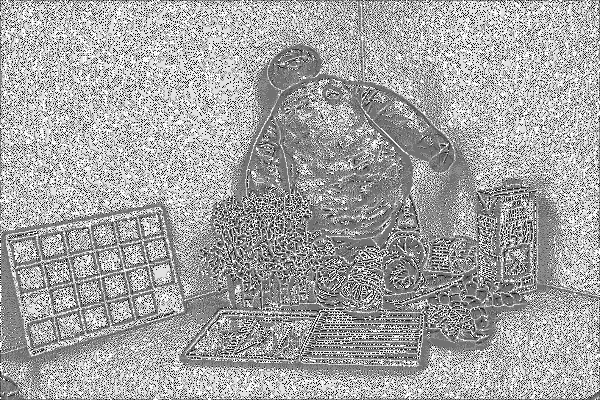
\includegraphics[width=.8\linewidth]{picture/LLIE/My Architecture/Edge Detection/normal00269_lbp}
				\captionsetup{font=scriptsize}
				\label{fig: GT_lbp1}	
				\caption*{GT LBP}
			\end{minipage}
			\captionsetup{font=scriptsize}
			\caption{
				\label{fig: LLI Structure Information1}
				LLI with noise and GT Structure Information
			}
		\end{figure}
	\end{frame}
	
		\begin{frame}
		\begin{figure}
			\centering
			\begin{minipage}{\textwidth}
				\centering
				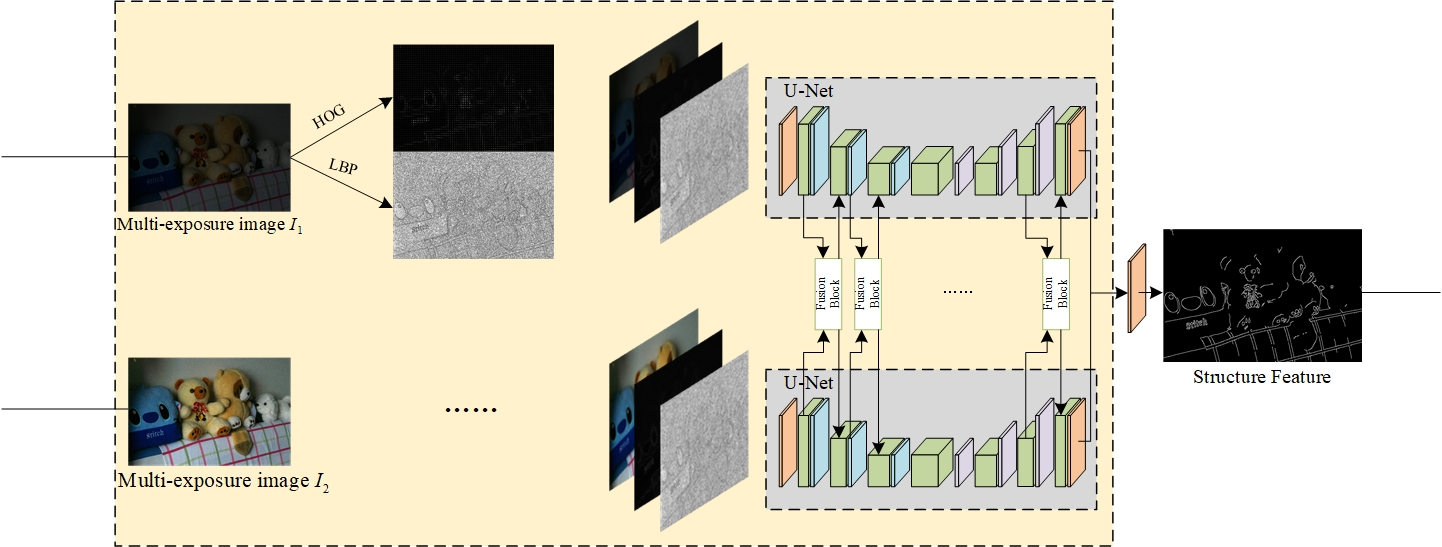
\includegraphics[width=\linewidth]{picture/LLIE/My Architecture/Edge Detection Network}
				\captionsetup{font=scriptsize}
				\label{fig: Edge Detection Network}	
				\caption{Edge Detection Network}
			\end{minipage}
		\end{figure}
	\end{frame}
	
	\section{Experimental Plan}
	
	\subsection{Dataset}
	
	\begin{frame}
		
		% 实验的过程中,确保所有的实验在相同的硬件和软件环境下进行,并且为了确保结果的可靠性,可能需要多次运行实验并取平均值。我们主要基于 PyTorch 进行模型的搭建、训练和评估,使用 Matplotlib 库用于绘制图标和注意力图。基于scikit-image 库计算PSNR、SSIM 等评价指标。
		
		\begin{itemize} 
			\item \textbf{Low-light Dataset}
		\end{itemize}
		
		\begin{table}[!htbp]
			\centering
			\tiny
			%\resizebox{\textwidth}{!}{ %按照宽度调整调整表格大小
				\begin{tabular}{>{\centering\arraybackslash}m{3cm}|c|c|c|c}
					
					\hline
					
					\textbf{Name} & \textbf{Number} & \textbf{Format} & \textbf{Real/Syn} & \textbf{Video} \\
					
					\hline
					
					LOL\textcolor{blue}{\citep{wei2018deep}} & 500 & RGB & Real & \\
					
					SCIE\textcolor{blue}{\citep{cai2018learning}} & 4,413 & RGB & Real & \\
					
					VE-LOL-L\textcolor{blue}{\citep{jiang2019learning}} & 2,500 & RGB & Real+Syn & \\
					
					MIT-Adobe FiveK\textcolor{blue}{\citep{bychkovsky2011learning}} & 5,000 & Raw & Real & \\
					
					SID\textcolor{blue}{\citep{wei2018deep}} & 5,094 & Raw & Real & \\
					
					DRV\textcolor{blue}{\citep{chen2019seeing}} & 202 & Raw & Real & \checkmark  \\
					
					SMOID\textcolor{blue}{\citep{jiang2019learning}} & 179 & Raw & Real & \checkmark  \\
					
					\hline
					
				\end{tabular}
				%}
			\captionsetup{font=scriptsize} %设置标题字体与表格字体一致
			\caption{\label{tab: Paired_training_datases}
				Summary of paired training datasets. 'Syn' represents Synthetic.} %表格的标题
			
		\end{table}
	\end{frame}
	
	\subsection{Train}
	
	\begin{frame}
		\begin{itemize}
			\item \textbf{Train}
			
			\checkmark Baseline Model
			% 基线模型: 首先,训练基线模型(即完整的并行模型,包含完整的CNN 和Transformer 分支)。
			
			\checkmark Ablation Study
			% 消融研究: 接着,训练去除Transformer 分支的模型,以进行消融实验。
		\end{itemize}
		
		\begin{itemize}
			\item \textbf{Performance Evaluation}
			
			\checkmark MSE
			% 均方误差
			
			\checkmark PSNR
			% 峰值信噪比
			
			\checkmark SSIM
			% 结构相似性指数
			
			\checkmark LPIPS
			% 感知图像质量评估
		\end{itemize}
		
		\begin{itemize}
			\item \textbf{Results analysis and reporting}
			
			\checkmark All experimental results were compiled into tables or graphs.
			% 数据整理: 将所有实验结果整理成表格或图表。
			
			\checkmark Analysis of differences
			% 分析: 分析不同数据集和不同模型配置(如有/无Transformer分支) 的性能差异。
		\end{itemize}
				
	\end{frame}
	
	
	
	\begin{frame}[plain,c]
		\begin{center}
			\Huge Thank you !
		\end{center}
	\end{frame}
	
	\appendix
	\begin{frame}[allowframebreaks]{References}
		\tiny
		%\bibliographystyle{unsrt}
		\bibliographystyle{elsarticle-harv}
		\bibliography{reference}
		%\bibliographystyle{plainnat}
	\end{frame}
	
\end{document}
